\documentclass{article}
\usepackage{graphicx}
\usepackage{float}
\usepackage{amsmath}
\usepackage{amsfonts}
\usepackage{amssymb}
\usepackage{hyperref}
\usepackage{esint}
\usepackage[utf8]{inputenc}
\usepackage[a4paper, portrait, margin=0.75in]{geometry}
\setlength\parindent{0pt}
\usepackage[italian]{babel}



\hypersetup{
    colorlinks=true,
    linkcolor=black,
    filecolor=magenta,
    urlcolor=blue,
    pdftitle={Tecnologie internet},
    pdfpagemode=FullScreen,
}


\begin{document}
    \author{dmotrio}
    \title{Big Data e Business Intelligence}
    \date{25 Gennaio 2022}

    \maketitle
    \tableofcontents

    \listoffigures
    \listoftables


    \section{Introduzione all'intelligenza artificiale}

Gli obiettivi di questo corso:
\begin{itemize}
    \item Capire i dati
    \item Visualizzazione de dati
    \item rappresentazione dei dati
    \item Estrazione della conoscenza
    \item Ingegnerizzazione dei dati
    \item Analsi predittiva
\end{itemize}

\subsection{Introduzione ai Big Data}
I big data sono quei dati che presentano una o più delle seguenti proprietà:
\begin{itemize}
    \item \textbf{Volume}: grandi quantità di dati
    \item \textbf{Varietà}: eterogeneità dei dati per tipologia, struttura, fonte, ecc
    \item \textbf{Velocità}: Dati che vengono generati con grande velocità
    \item \textbf{Veridicità}: dati sconnessi, mancanti, inconsistenti
\end{itemize}

Possoiamo categorizzare i dati in base alla loro struttura:
\begin{itemize}
    \item Dati strutturati
    \item dati non strutturati
    \item dati semi-strutturati
\end{itemize}

\subsubsection{Dati strutturati}
I dati strutturati sono quei dati rappresentabili in tabella, DB, CSV.
\subsubsection{Dati non strutturati}
Non rappresentabili in tabelle.
ES:
PDF, video, audio, immagini, ecc

\subsubsection{Dati semi-strutturati}
Dipendentemente dalla task che si vuole svolgere, si possono trattare i dati come
strutturati, semi-strutturati o non strutturati.


\subsubsection{Qualità dei dati}
La qualità dei dati dipende da:
\begin{itemize}
    \item \textbf{Completezza}
    \item \textbf{Consistenza}
    \item \textbf{Accuratezza}
    \item \textbf{Assenza di duplicati}
    \item \textbf{Integrità}
\end{itemize}

\subsubsection{Fonti dei dati}
Dati interni:
\begin{itemize}
    \item produzione
    \item tranazioni o statistiche di utilizzo
    \item vendite
    \item human resource manager(HR)
    \item customer relationship manager(CRM)
\end{itemize}

Dati esterni sono i dati ottenibili pubblicamente, dati di forum, social network, ecc.

\subsubsection{Dati operazionali}
In una organizzazione ci sono tre tipologie di individui interessati ai dati:
\begin{itemize}
    \item \textbf{Manager}: deve prendere decisioni
    \item \textbf{Operation staff}: motore di ogni singola tasks e fornisce dati interni
    \item \textbf{Data scientist}: responsabile di gestire, analizzare e preparare i dati per il manager e lo staff operativo
\end{itemize}

Visto che questi dati sono tantissimi, si usano Enterprise Resource Planning(\textbf{ERP}) software.

Solitamente i DB utilizzati in questi sistemi, sono disegnati per essere \textbf{OLTP}
(On Line Transaction Processing).
Sono incentrati sulla lettura de dati e non sulla loro analisi.

\subsubsection{I dati operazionali sono un po' meh per le analisi}
Di solito si usano i \textbf{Data Werehouse}, dati fatti su misura che contengono dati consistenti e interessanti per l'analisi.


I Data Werehouse sono il punto di partenza della \textbf{Business intelligence}

\subsubsection{Business Intelligence}
Sistema di modelli, metodi, processi, persone e strumenti che rendono possibile la raccolta regolare ed organizata del patrimonio
di dati generato da una organizzazione.
Attraverso elaborazioni, analisi o aggregazioni, permette:
\begin{itemize}
    \item Trasformazione di informazioni
    \item Conservazione
    \item Reperibilità
    \item Presentazione in forma semplice, flessibile ed efficiente
\end{itemize}

\subsubsection{Ragioni per il fenomeno dei big data}
\begin{itemize}
    \item Computer avanzati
    \item DB non relazionali più performanti
    \item Progresso con il Machine Learning
    \item Progetti open-source
\end{itemize}
\subsubsection{Principali software open-source}
\begin{itemize}
    \item Hadoop
    \item Spark
    \item Python
\end{itemize}

\subsubsection{ML per l'estrazione del'informazione}
ML è un campo di studi dove non si programma per svolgere una task specifica, un 
sistema di ML si \textbf{"allena"} sulla task da eseguire.
Il sistema di ML crea esperienza sulla base degli esempi,
trova patter regolari fra i vari casi e in base all'esperienza acquisita
può prendere decisioni per il futuro.

\subsubsection{Chi è il Data Scientist}
Persona che ha il compito di analizzare i dati con tecniche avanzate,
solitamente con abbastanza conoscenza del dominio e buone soft-skills.

Forte background in:
\begin{itemize}
    \item Computer Science
    \begin{itemize}
        \item DB e SQL
        \item Hadoop
        \item Spark
        \item NoSQL
        \item Python, java, ecc
        \item Artificial Intelligence
    \end{itemize}
    \item Machine Learning
    \item Statistica
\end{itemize}




    \section{Elementi di scienza dei dati}

\subsection{Analisi descrittiva}
Grafici e numeri vengono usati per riassumere e processare i dati trasformando l'informazione.

\begin{itemize}
    \item Si hanno troppi dati ed è difficile trarre conclusioni
    \item riassumere i dati senza perdere informazioni
    \item riassumere dipende dal task
    \item la visualizzazione dei dati è una delle parti più importanti dell'anailisi descrittiva
\end{itemize}

\subsubsection{Classificazione delle variabili}
\begin{itemize}
    \item Categoriche: (male, bene, buono, ottimo)
    \item Numeriche
    \begin{itemize}
        \item discrete
        \item continue(misurzioni del mondo reale)
    \end{itemize}
\end{itemize}

\subsubsection{Livelli di misurazione}
Per estrarre conoscenza dai dati categorici, bisogna associare loro un valore.
Un'altra Classificazione dei dati è:
\begin{itemize}
    \item Dati qualitativi: non c'è una misura fra la differenza di due dati(maschio femmina)
    \item dati quantitativi: la differenza fra due dati ha un senso(3 banane)
\end{itemize}

\begin{figure}[H]
    \centering
    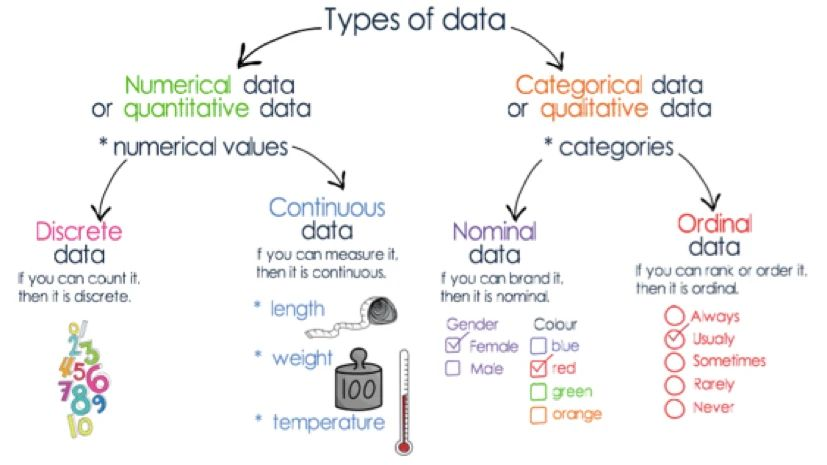
\includegraphics[width=0.7\linewidth]{imgs/1 - dati}
    \caption{Tipi di dati}
    \label{fig:tipi_di_dati}
\end{figure}

\subsection{Descrizione numerica dei dati}
\subsubsection{Misura della tendenza centrale}
I dati tendono ad un valore e usiamo:
\begin{itemize}
    \item media aritmetica
    \item mediana
    \item moda
\end{itemize}

\subsubsection{Media}
\begin{equation}
    M_a = \frac{1}{n}\sum_{i=1}^{n}x_i
    \label{eq:media}
\end{equation}
\subsubsection{Mediana}
Se i numeri presi in considerazione sono dispari, una volta ordinati, si prende quello centrale.
Se i numeri sono dispari, dopo l'ordinamento, si prende il numero successivo a quello che sarebbe il centrale.

\subsubsection{Moda}
La moda è l'elemento più frequente.

\subsubsection{Misura di dispersione: Varianza}
Qaunto i dati si discostano dalla media.
\begin{equation}
    \sigma_X^2 = \frac{\sum_{i}(x_i - \mu_X)^2}{n}
    \label{eq:varianza}
\end{equation}

\subsubsection{Misura di dispersione: Deviazione standard}
Togliendo la radice quadrata:
\begin{equation}
    \label{eq:deviazione_standard}
    \sigma = \sqrt[2]{\frac{\sum_{i=1}^{N}(X_i - \mu)^"}{N}}
\end{equation}

\subsubsection{Relazione fra due variabili: covarianza}
\begin{equation}
    cov(X,Y) = \frac{\sum{(X_i -
    \overline{X})(Y_j
    - \overline{Y})}}
    {n}
    \label{eq:covarianza}
\end{equation}

\subsubsection{Relazione fra due variabili: correlzione di pearson}
\begin{equation}
    \rho_{X,Y} = \frac{cov(X,Y)}{\sigma_X\sigma_Y}
    \label{eq:pearson}
\end{equation}




























    \section{Business intelligence: generalità}
Trasformare i dati grezzi in informazioni
utilizzabili, da distribuire e condividere, creando così una conoscenza
collettiva della propria impresa.

\begin{itemize}
    \item E’ un processo analitico che trasforma i dati in informazioni
    a supporto della presa di decisioni ottimizzato da un
    insieme di tecnologie
    \item Con
    il fine di Migliorare i processi decisionali, di
    comunicazione e coordinamento delle interdipendenze
    aziendali, razionalizzare e ottimizzare il processo di Conoscenza
    creazione, gestione, diffusione e condivisione della
    conoscenza
\end{itemize}
\subsection{Business Intelligence: Leggere i dati per guidare le decisoni}

Fa uso di flussi di dati di qualsiasi dimensione per analizzare e visualizzare informazioni cruciali,
in relazione all'utilizzo che se ne intende fare.

Le aziende possono fare uso della BI per infromarsi sulle opzioni disponibili, permettendo di
migliorare la resa economica, l'efficienza, ecc.

La BI cerca di indivisuare e rendere percepibili i segnali nascosti contestualizzandoli.

Con la BI è possibile:
\begin{itemize}
    \item raccogliere dati
    \item classificare le informazioni
    \item analizzare i risulatati
    \item realizzare modelli predittivi
\end{itemize}

La BI si avvale di:
\begin{itemize}
    \item piattaforme dedicate
    \item modelli matematici, statistici e di analisi
    \item verifica dei risulatati
    \item esperti in materia
\end{itemize}

Si tratta di un percorso di valutazione supportato da strumenti di data visualizzation.
La BI è la chiave di lettura ottimale per capire cosa è successo e cosa sta succedendo,
offrendo soluzioni che aiutano a identificare schemi di comportamento significativi
e correlazioni tra le variabili entro un complesso insieme di dati, strutturati e non,
storici, attuali e potenziali.


Per avere una visione globale dell'azzienda, bisogna organizzare i dati in un unico rapporto.
Gli strumenti:
\begin{itemize}
    \item i report
    \item la dashboard(rappresentazioni dei dati graficamente)
    \item la dashboard rappresentano i \textbf{KPI}(Key Performance Indicator)
\end{itemize}

\subsubsection{Componenti della BI}
\begin{itemize}
    \item Dati: nozioni grezze
    \item informazioni: informazioni ottenute dai dati
    \item conoscenza: identificazioni di relazioni causa-effetto tra le infromazioni attraverso
    l'esperienza
\end{itemize}

\subsubsection{Gestione della conoscenza}
Creazione, raccolta e classificazione di informazioni provenienti da varie fonti
di dati che vengono distribuite ai vari utenti sulla base degli specifici interessi tramite
mezzi e strumenti diversi.

\subsubsection{Utenti nella BI}
\begin{enumerate}
    \item utente di alto livello: vista ampia e prende decisoni
    \item utenti specializzati: eseguono analisi dei dati
    \item lavoratori con necessità di report di base
    \item lavoratori senza report
\end{enumerate}

\begin{figure}[H]
    \centering
    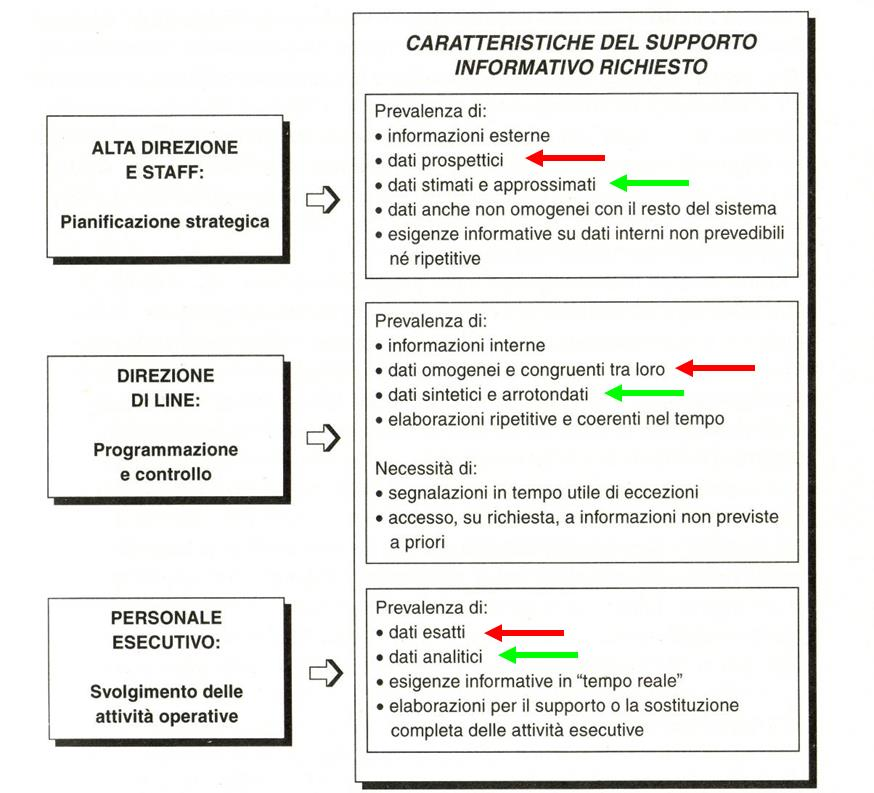
\includegraphics[width=0.4\linewidth]{imgs/2 - utenti BI}
    \label{fig:utenti_BI}
    \caption{Utenti nella BI}
\end{figure}


\subsection{Il valore della conoscenza}
\begin{figure}[H]
    \centering
    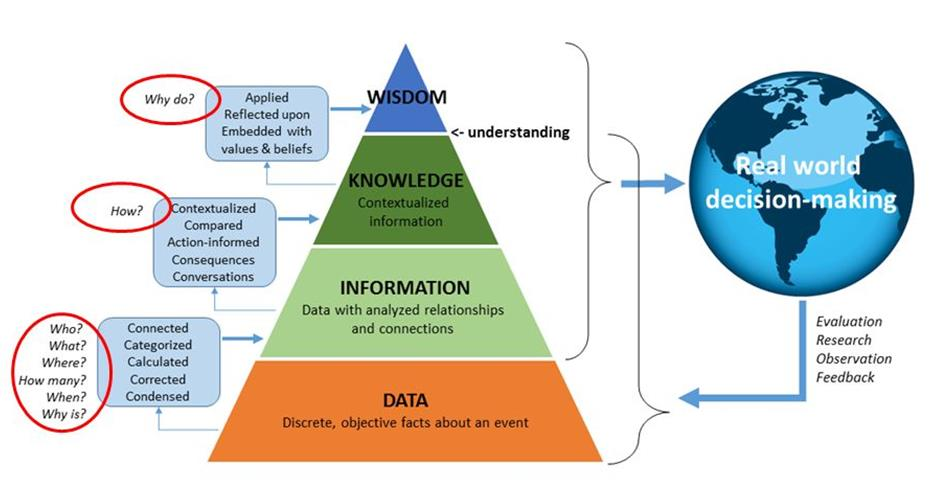
\includegraphics[width=0.6\linewidth]{imgs/3 - La piramide di DIKW}
    \label{fig:piramide_DIKW}
    \caption{Piramide di DIKW}
\end{figure}
\begin{itemize}
    \item Dati: nozioni grezze
    \item Informazioni: rappresentazione dei fatti (dati)
    organizzati in modo da essere comprensibili e
    significativi per l’utente destinatario
    \item Conoscenza: il collegamento fra più informazioni quali p.e.,
    l’identificazione di relazione causa-effetto
    tra informazioni attraverso esperienza, relazioni sociali etc.
    \item saggezza: capacità di aumentare l'efficacia. La saggezza aggiunge valore, il che
    richiede la funzione mentale che chiamiamo giudizio. I valori etici ed estetici che
    questo implica sono intrinseci all'attore e sono unici e personali. (Russell Ackoff)
\end{itemize}

\subsubsection{Ciò che genera conoscenza}
\begin{enumerate}
    \item Descriptive Analytics: l’insieme di strumenti orientati a descrivere la
    situazione attuale e passata dei processi aziendali e/o aree funzionali. Tali
    strumenti permettono di accedere ai dati secondo viste logiche flessibili e
    di visualizzare in modo sintetico e grafico i principali indicatori di
    prestazione
    \item Predictive Analytics, strumenti avanzati che effettuano l’analisi dei dati
    per rispondere a domande relative a cosa potrebbe accadere nel futuro;
    sono caratterizzati da tecniche matematiche quali regressione, forecasting,
    modelli predittivi, ecc
    \item Prescriptive Analytics, applicazioni big data avanzate che, insieme
    all’analisi dei dati, sono capaci di proporre al decision maker soluzioni
    operative/strategiche sulla base delle analisi svolte
    \item Automated Analytics, capaci di implementare autonomamente l’azione
    proposta secondo il risultato delle analisi svolte
\end{enumerate}

\subsection{Dati di qualità per essere affidabili}

I problemi:
\begin{itemize}
    \item dati in più posti
    \item dati non formattati per anali complesse
    \item diversi lavoratori operano su dati in maniera diversa
    \item quali dati dovrebbero essere esaminati
    \item interazione degli utenti
\end{itemize}

\subsection{Consolidamento dei dati}

\subsubsection{Pulizia dei dati}
I dati potrebbero essere incoerenti.
\subsubsection{Creare dati di qualità}
I dati puliti facilitano analisi più accurate.

\subsubsection{Estrazione, trasformazione e caricamento(ETL)}
Il processo di spostamento dei dati dai sistemi di origine, il consolidamento in una posizione centrale e la
correzzione delle incoerenze si chiama estrazione, trasformazione e consolidamento.

Il processo di ETL richiede l'$80\%$ del tempo.

\subsubsection{Datawarehouse}
I dati possono stare in posti diversi e fromati diversi, DB relazionali, fogli Excel ecc.
I Datawerehouse permettono di ottenere un layer di astrazzione, separando la provenienza dei dati dal loro utilizzo.

\begin{figure}[H]
    \centering
    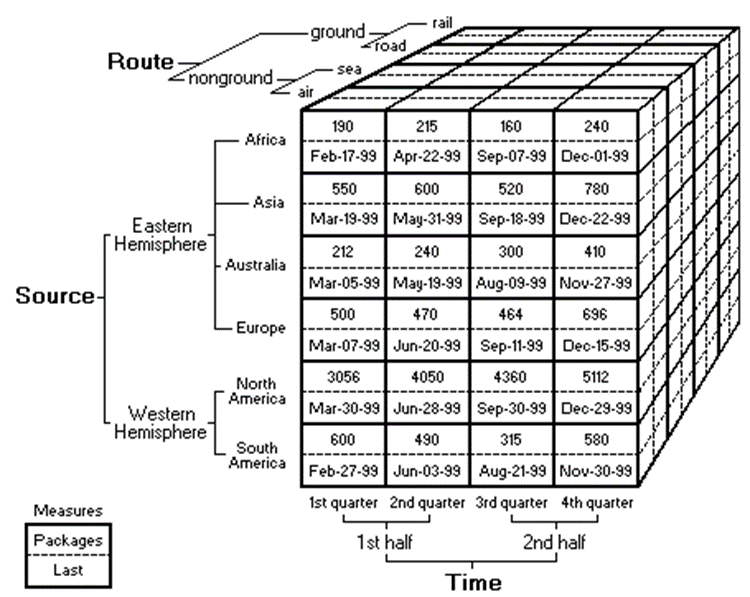
\includegraphics[width=0.4\linewidth]{imgs/4 - DWH}
    \label{fig:DWH}
    \caption{Cubo che compone il DWH}
\end{figure}

Il cubo è il componente base di un data werehouse, un DWH può contenere più cubi.


\subsubsection{OLAP}
Permette l'analisi dei dati su strutture che rendono le operazioni veloci e flessibili.

Tre categorie principali:
\begin{itemize}
    \item MOLAP
    \begin{itemize}
        \item più usati
        \item ha un motore specifico per l'analisi
        \item crea le dimensione con un misto di dettaglio e astrazione
        \item veloce
    \end{itemize}
    \item ROLAP
    \begin{itemize}
        \item lavora sui DB relazionali
        \item minor spazio su disco e ram
        \item più lento
    \end{itemize}
    \item HOLAP
    \begin{itemize}
        \item lavora con DB relazionali
        \item più veloce dei ROLAP
        \item più scalabile dei MOLAP
    \end{itemize}
\end{itemize}

Le principali operazioni negli OLAP sono:
\begin{itemize}
    \item PIVOTING
    \begin{figure}[H]
        \centering
        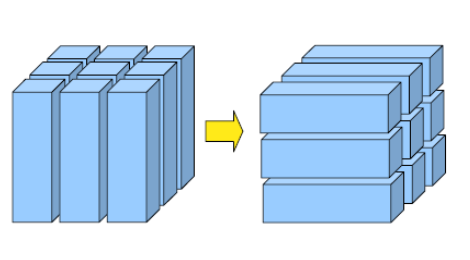
\includegraphics[width=0.2\linewidth]{imgs/5 - pivoting}
        \label{fig:pivoting}
        \caption{Pivoting}
        è l'operazione di rotazione delle dimensioni di analisi. È un'operazione
        fondamentale per analizzare totali ottenuti in base a dimensioni diverse o
        se si vogliono analizzare aggregazioni trasversali.
        La tabella pivot è la reportistica che risulta da una query OLAP elaborata
        su dati organizzati all'interno di un ipercubo OLAP
    \end{figure}
    \item SLICING
    \begin{figure}[H]
        \centering
        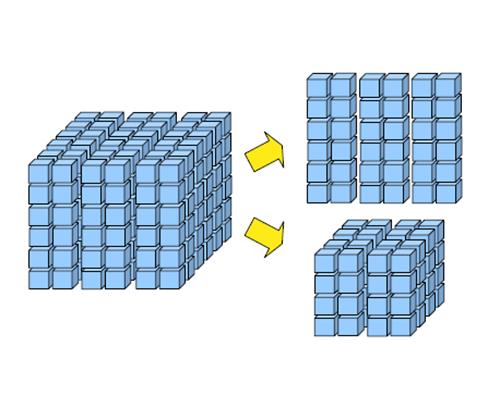
\includegraphics[width=0.2\linewidth]{imgs/6 - slicing - dicing}
        \label{fig:slicing-dicing}
        \caption{Slicing e Dicing}
        Si fissa uno specifico valore per una delle
        dimensioni del "cubo", estraendo quindi una
        "fetta" e ottenendo un nuovo cubo con una
        dimensione in meno rispetto a quello di
        partenza
    \end{figure}
    \item DICING
    Si focalizza l’analisi su un sottoinsieme del
    "cubo" avente particolare interesse per
    l'analista
    \item DRILL-DOWN
    \begin{figure}[H]
        \centering
        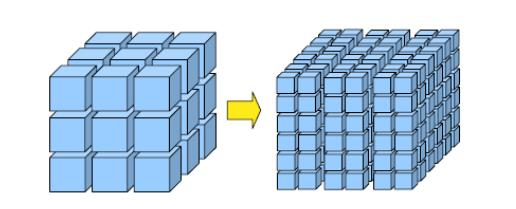
\includegraphics[width=0.3\linewidth]{imgs/7 - drill down}
        \label{fig:drill_down}
        \caption{Drill-down}
    \end{figure}
    è l'operazione di "esplosione" del dato nelle sue determinanti.
    L'operazione di drill-down può essere eseguita seguendo due diversi
    percorsi: la gerarchia costruita sulla dimensione di analisi (p. es.:
    passaggio dalla famiglia di prodotti all'insieme dei prodotti che ne fanno
    parte) oppure la relazione matematica che lega un dato calcolato alle sue
    determinanti (p. es.: passaggio dal margine al ricavo e costo che lo
    generano).
\end{itemize}


\subsubsection{Data mining}
Estrazione di conoscenza da banche grandi banche dati tramite algoritmi che individuano
le associazioni nascoste tra le informazioni e le rendono disponibili.

Con il data mining si intende l'applicazione di una o più tecniche che consentono l'esplorazione
di grandi quantità di dati, con l'obbiettivo di individuare le informazioni più significative.


Un processo di base consiste in:
\begin{enumerate}
    \item definizione dell'obbiettivo
    \item indivisuazione delle fonti
    \item estrazione dei dati
    \item pre-processing
    \item data mining
    \item interpretazione
    \item reppresentazioni dei risultati
\end{enumerate}

Tipologia di problemi ai quali il data mining fonisce una risposta:
\begin{itemize}
    \item Classificazione: definizione delle caratteristiche del data set
    \item Clustering: identificazione delle affinità che definiscono i gruppi
    \item Sequencing: identificazioni delle correlazioni in un periodo definitp
    \item associazione: identificazione delle correlazioni tra comportamenti
    \item Previsione: identificazioni di trend
\end{itemize}

\begin{figure}[H]
    \centering
    
\includegraphics[width=0.7\linewidth]{imgs/8 - dataming}
    \label{fig:data_mining_domande}
    \caption{Domande DM}
\end{figure}

\subsection{Osseviamo i dati}
Attualmente ci sono quantità di dati quasi infiniti prodotti quotidianamente,
bisogna darci un senso\ldots

\subsubsection{Le fonti}

\begin{itemize}
    \item Interne
    Fonti operazionali, dati sul business interno ecc
    \item Esterne
    analisi dei sentiment, ecc
\end{itemize}
\subsubsection{Aspetto}

\begin{itemize}
    \item Dati quantitativi
    descritti tramite numeri
    \item Dati qualitativi
    non rappresentati dal valore numerico
\end{itemize}

\subsubsection{Struttura}
\begin{itemize}
    \item Dati strutturati
    dati ordinati in una struttura
    \item Dati non strutturati
    formato libero
    \item Dati semi strutturati
\end{itemize}

Il $90\%$ dei dati sono in un formato difficile per l'elaborazione.

\subsubsection{I quattro livelli dei dati}
\begin{itemize}
    \item Livello nominale
    Dati descritti unicamente per nome e categoria.
    Per trovare il centro dei dati si considera la moda.
    \item livello ordinale
    Esiste unìordine di valutazione, utile all'ordinamento e al confronto.
    SI utilizza la mediana.
    \item livello degli intervalli
    i dati di questo tipo consentono di eseguire sottrazioni fra i punti dei dati.
    Si usa la media.
    \item livello dei rapporti
    I dati al livello intervalli non hanno un valore nullo o zero, sui dati dei rapporti si possono fare
    moltiplicazioni e divisioni.
    La media imane topppp.
\end{itemize}


\subsection{Dara science Vs Business Intelligence}
\subsubsection{BI}
\begin{itemize}
    \item fondamentale l'uso di tecnologie e processi dalle aziende per l'anili dei dati
    \item esegue la conversione da dati grezzi a informazioni
    \item anali dei dati strutturati per aprendere conoscenza
    \item supporta il processo decisionale basato sui fatti
    \item ha un impatto direttosulle decisione delel aziende
    \item nuove opportunità per l'azienda
\end{itemize}

\subsubsection{Data science}
\begin{itemize}
    \item fondamentale un campo in cui la conoscenza venga estratta dai dati usando vari metodi e algoritmi
    \item combinazione di vari strumenti matematici, algoritmi, statistica, e tecnologie di apprendimento automatico
    \item sia dati strutturati che non
    \item implica lo studio delle tendenze attuali e prevede le future
\end{itemize}


\subsubsection{Analisi con BI}
\begin{itemize}
    \item BI lavora su una formula preesistente
    \item l'azienda contatta un esperto di BI con i dati e le formule e si aspetta un risultato definito
\end{itemize}
\subsubsection{Anali con DS}
\begin{itemize}
    \item Si parte da una domanda
    \item non si utilizza la solita formula
    \item La Sciena dei dati cerca di anticipare il futuro
\end{itemize}

\begin{figure}[H]
    \centering
    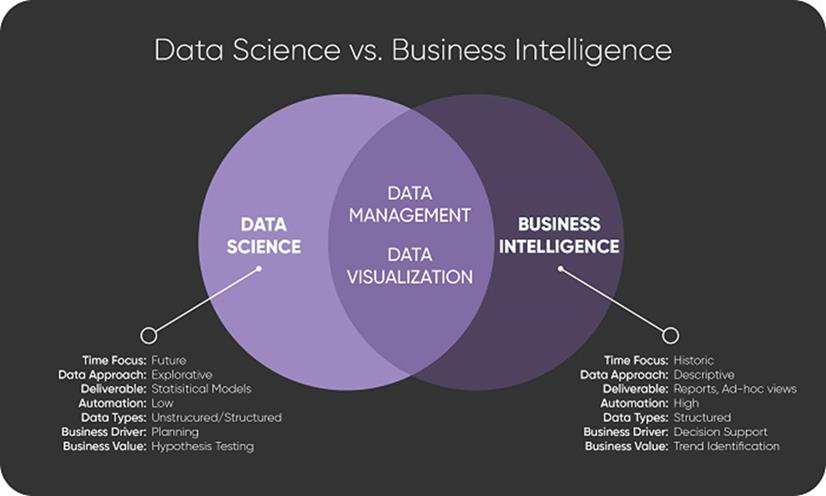
\includegraphics[width=0.8\linewidth]{imgs/10 - BI VS DS}
    \label{fig:data_science_vs_business_intelligence}
    \caption{Data Science VS Business Intelligence DM}
\end{figure}

    \section{Intelligenza artificiale}

\subsection{Intelligenza artificiale}
I principali settori dell'IA sono:
\begin{itemize}
    \item Emulazione dei processi logici(conoscenza inserita dal progettista)
    \item Apprendimento automatico(Machine learning)
\end{itemize}

Le capacità richieste ad una IA sono:
\begin{itemize}
    \item Apprendere informazioni del mondo mediante un sistema di percezione(telecamere, dati, ecc)
    \item Dedurre sul mondo attraverso processi di inferenza
\end{itemize}

\subsubsection{Intelligenza artificiale e Intelligenza}
Con l'intelligenza artificiale si entra in un settore complicato, è difficile formulare una definizione di
Intelligente poichè spesso associato a umano, e tante altre domande di questo genere.

Visto che non sappiamo come funzioni l'intelligenza e la conoscenza,
per valutare una IA, si ricorre ad un test comportamentale.

\subsubsection{Test di Touring}
Un computer è da considerarsi intelligente
se, nell'interazione a distanza con un
essere umano, non è in grado di
distinguere se sta interagendo con un
uomo o una macchina.

Questa teoria spesso superata e riformulata, porta a definizione di AI debole(simula il pensiero) ed AI forte
(PENSA).

\subsubsection{AI: forte VS debole}
Non è comunemente accettato il fatto che la conoscenza umana possa essere replicata in una macchina
e altre idee simili.
\begin{itemize}
    \item le macchine pensano davvero o eseguono gli ordini?
    \item le macchine possono imparare a pensare?
    \item le macchine possono essere programmate per provare emozioni?
\end{itemize}

L'IA \textbf{forte} è una frma teorica per descrivere una certa mentalità dello sviluppo di sistemi AI.
Punta a creare intelligenze indistinguibili da quella umana.

In questo caso si potrebbe direr che la IA possa avere una coscienza(globalmente accettato?).

Secondo i fautori della IA \textbf{debole}, è impossibile attualmente creare una AI forte principalmente per la
assente definizione esplicita della intelligenza e comprensione.
I sostenitori della IA debole, affermano che una IA non debba avere una coscenza.


\begin{figure}[H]
    \centering
    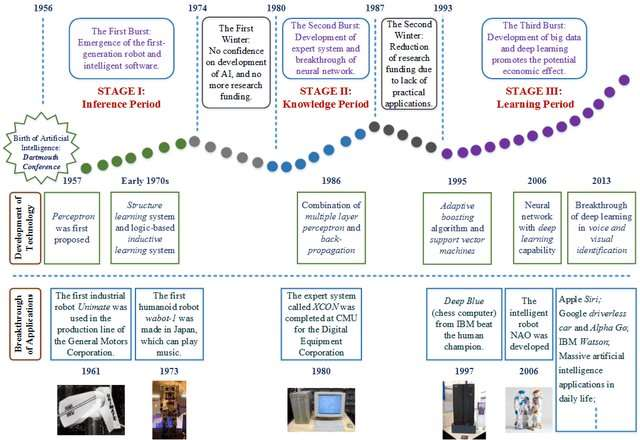
\includegraphics[width=1\linewidth]{imgs/11 - storia IA}
    \caption{Storia IA}
    \label{fig:storia_ia}
\end{figure}




    \section{Tecniche per AI}
\begin{figure}[H]
    \centering
    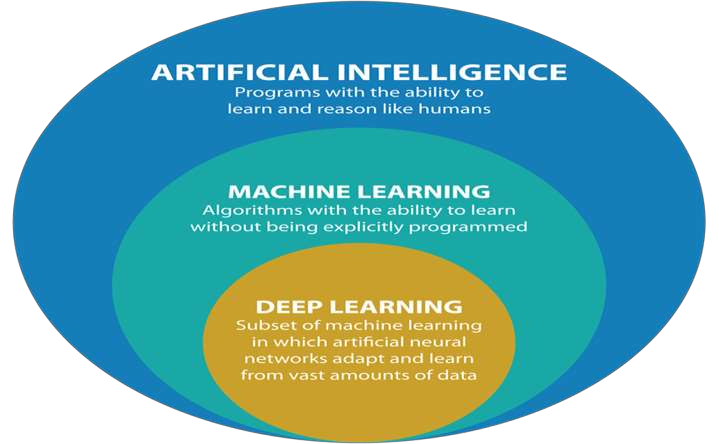
\includegraphics[width=0.5\linewidth]{imgs/12 - campi dell'ai}
    \caption{Branche della AI}
    \label{fig:campi_ai}
\end{figure}

Attualmente la AI si occupa di:
\begin{itemize}
    \item identificazione di modelli
    \item idedntificazioni algoritmi
\end{itemize}


\subsection{Costruzione di una IA}
\subsubsection{Conoscenza}
Conoscenza come:
\begin{itemize}
    \item informazioni(nozioni)
    \item conoscenza(cultura, dottrina)
    \item competenza(abilità, tecnica)
\end{itemize}

L'esperienza può venire sia da esperienze dirette che indirette.

Nei computer la conoscenza non è strettamente legata all'informazione, moli di dati non forniscono 
alcuna informazione.

\textbf{La conoscenza è informazione disponibile per un'azione razionale.}
Però non sempre una sceltarazionale è legata all'inferenza e viceversa.

\subsubsection{Agire razionale}
Gli individui agiscono sulla conoscenza e sulle percezioni del mondo attraverso ragionamento:
\begin{itemize}
    \item deduttivo: dalla premessa alla conclusion
    \item abduttivo: dagli effetti alle possibili cause
    \item induttivo: da fatti specifici a regole generali
\end{itemize}
per produrre nuova conoscenza.

\subsubsection{Due approcci differenti}
\begin{itemize}
    \item top down o simbolico
    La conoscenza è rappresentata da simboli. Vengono utilizzate la
    logica e la capacità di fare inferenze
    \item bottom up o subsimbolico
    Non esiste una rappresentazione esplicita della conoscenza.
    Vengono utilizzate reti neurali, approcci evolutivi, ecc
\end{itemize}

\begin{figure}[H]
    \centering
    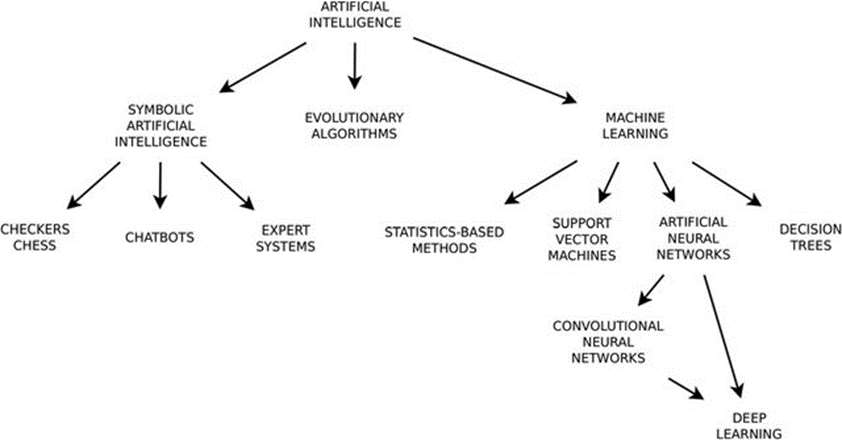
\includegraphics[width=0.8\linewidth]{imgs/13 - ai}
    \caption{Tecniche per AI}
    \label{fig:ai_tecniche}
\end{figure}

\subsection{Approccio simbolico}
Alla AI viene fornito una descrizione del dominio in linguaggio formale, per attingere
a questa base di conoscenza e inferire nuova conoscenza(o azioni da intraprendere).

\subsubsection{Logica}
La logica fornisce strumenti formali per:
\begin{itemize}
    \item Esprimere inferenze
    \item dedurre le conseguenze
    \item studiare la verità o la falsità
    \item stabilire la coerenza e la validità
\end{itemize}


La logica si basa sul ragionamento deduttivo.
In logica, la conoscenza iniziale è indicata come assiomi. Le nuove
conoscenze derivate dagli assiomi sono chiamate teoremi.

Per inferire nuovi teoremi si usa la \textbf{regola di inferenza}.(usando il simbolo "$\Rightarrow)$")

Esempio:
$A$ è vero, $B$ è vero $\Rightarrow$ C è vero.

In generale, in logica si studia la relazione tra le formule di un sistema logico-simbolico
in cui:
\begin{itemize}
    \item il linguaggio delle formule è definito con precisione
    \item il significato delle formule è stabilito in modo univoco
\end{itemize}

La logica moderna ha il compito si rappresentare in modo formale la corrispondenza tra espressioni
linguistiche e significato inteso.
Ls formalizzazione(astrazione) è una sorta di compressione delle informazioni, con ampia
perdita di dettaglio e guadagno di precisione.

\subsection{Logica proposizionale}
\subsubsection{La base}
La \textbf{logica} è un linguaggio formale per rappresentare informazioni e dedurre conclusioni,
la \textbf{sintassi} definisce le proposizioni ammissibili dal linguaggio,
la \textbf{semantica} definisce il "significato" dell'asserzione.

\subsubsection{Implicazione}
\begin{equation*}
    KB \models \alpha
\end{equation*}

La conoscenza KB implica $\alpha$, se $\alpha$ è vera allora KB sono verificati.


\subsubsection{Sintassi logica proposizionale}
\begin{itemize}
    \item definisce frasi ammissibili
    \item le frasi atomiche sono fatte da un singolo simbolo
    \item questi simboli possono essere veri o falsi
    \item le frasi complesse sono un insieme di frasi semplici
\end{itemize}

Connettivi:
\begin{itemize}
    \item negazione con sengo -
    \item and $\wedge$
    \item or $\vee$
    \item implicazione $\Rightarrow$
    \item equivalenza $\Leftrightarrow$
\end{itemize}

\subsubsection{Semantica logica proposizionale}
\begin{itemize}
    \item la semantica definisce le regole per determinare la verità di una frase rispetto al modello
    \item nella logica proposizionale, il modello fissa la verità
    \item le frasi sono costrutite dalle frasi atomiche e dai 5 connettivi
\end{itemize}

Bisogna usare delle tabelle di verità.

\subsubsection{Limiti della logica proposizionale}
Troppo semplice, una merda.

\subsection{AI e ontologie, tecnologie semantiche}
\subsubsection{Logica descrittiva e ontologie}
i metodi semantici e le reti semantiche usano sitemi di logica descrittiva, adatta al ragionamento automatico.
\textbf{In AI, l'ontologia è una descrizione formale esplicita di un dominio di interesse.}


Quindi un ontologia è costituita da:
\begin{itemize}
    \item classi(concetti generali del dominio di interesse)
    \item relazioni tra queste classi
    \item proprietà assegnate a ciascun concetto, che ne descrivono vari tipi di attributi o proprietà
    \item restrizioni sulle proprietà
\end{itemize}

A partire dalle classi di ontologia, è possibile definire delle istanze, che rappresentano specifici oggetti
del mondo reale.

Knowledge base = Ontologia + insieme delle istanze delle classi.

Esistono ontologie specifiche(inerenti al dominio di applicazione) e generali.

Le ontologie organizzano tutti gli elementi della realtà in una gerarchia di categorie,
gli elementi padre passano i loro attributi ai figli(come nella programmazione a classi).

Esempio pizza:
\begin{figure}[H]
    \centering
    \includegraphics[width=0.8\linewidth]{imgs/14 - pizza ontologia eredità}
    \caption{Ontologia: Esempio della pizza}
    \label{fig:pizza}
\end{figure}

\subsubsection{Ontologia: termini ricorrenti}
\begin{itemize}
    \item Sussunzione: usata per creare gerarchie
    \item meronimia: descrive come si combinano i concetti
    \item vocabolario controllato: lista di termini numerati
    \item tassonomia: collezione di termini
    \item thesaurus: rete di termini
\end{itemize}
\subsubsection{Ontologia: operazioni tipiche}
\begin{itemize}
    \item costruire un modello ontologico
    \item eseguire il mapping tra concetti
    \item unire in un modello le informazioni
\end{itemize}
\subsubsection{Vantaggi delle ontologie}
\begin{itemize}
    \item permette la rappresentazione esplicita di modelli semantici
    \item abilitano l'applicazione di strumnti capaci di ragionamento
    \item adattamento a contesti differenti
    \item capacità di modellare domini che evolvono
\end{itemize}

\subsubsection{Ontologie: limiti}
\begin{itemize}
    \item difficoltà di rappresentare il problema
    \item avere uno standard
\end{itemize}

\subsection{IA: approccio sub-simbolico}
L'apprendimento deriva dall'esperienza.

\subsubsection{Comportamenti emergenti}
Nei sistemi complessi si parla di \textbf{compotamenti emergenti}, osservabili quando
l'attenzione si sposta dal singolo individuo alla collettività.

Spesso non rispecchiano il comportamento previsto.

Si cerca di programmare i singoli elementi dotandoli di far tendere il collettivo verso una direzione.

Si lascia poi che il sistema si organizzi.

\subsubsection{Ragionamento e apprendimento}
Il sistema intelligente deve saper ragionare e di acquisire nuova conoscenza in autonomia.

L'apprendimento è fondamentale per:
\begin{itemize}
    \item risolvere nuovi problemi
    \item non ripetere errori
    \item risolvere problemi in maniera più efficiente
    \item avere autonomia e adattarsi
\end{itemize}

\subsubsection{Apprendimento induttivo}
dato un insieme di esempi(campioni) di f, definsci una funzione h(ipotesi) che approssima f.

Si cerca di generalizzare le infromazioni per prevedere altre siteuazioni.

\subsubsection{Apprendimento da esempi}
Con l'apprendimento induttivo, gli esempi possono essere costruiti da:
\begin{itemize}
    \item descrizioni(pattern) di un'istanza di un fenomeno/problema da risolvere.
    \item insieme di coppie di dati
\end{itemize}

Per ottenere un buon esempio da dare in apprendimento, l'esempio deve essere rappresentativo del problema.

Abbastanza esempi??

\subsection{Inferenza in IA}
\subsubsection{Sistemi esperti}
Un sistema esperto è un sistema basato su regole di produzione che, a partire da alcuni dati, cerca
di dimostrare un'ipotesi.

\begin{enumerate}
    \item IF Meteo=‘Soleggiato’ AND Umidità=‘Bassa’ THEN Gioco
    \item IF Meteo=‘Soleggiato’ AND Umidità=‘Alta’ THEN Non Gioco
    \item IF Meteo= ‘Pioggia’ AND Vento = VERO THEN Non Gioco
    \item IF Meteo= ‘Pioggia’ AND Vento = FALSO THEN Gioco
    \item IF Meteo= ‘Nuvoloso’ THEN Gioco
    \item ELSE Gioco
\end{enumerate}

Prende una decisione sui fatti disponibili.

\subsubsection{Alberi decisionali}
Si può costruire un albero decisionale da una serie di esempi.

\subsubsection{Learnign = infering + memorizing}
durante l'apprendimento se un dato risulta utile, viene memorizzato.

Le inferenze possono essere deduttive o induttive.

Le inferenze possono essere divise in inferenze forti(conclusioni) o deboli(contingenti).

\subsection{Black box AI \& explainable AI}
I sitemi di ML possono funzioanre in questi due modi.


\subsubsection{Reti neurali artificiali: deep learning}
\begin{itemize}
    \item difficoltà a generalizzare
    \item scarso capacità di inferenza e gestione del agionamento logico
    \item difficile spiegare il loro comportamento
    \item difficoltà a ditinguere correzioni e causa-effetto
\end{itemize}

Explainable AI (XAI) studia il motivo per cui è stata presa una decisione
dall’AI in modo che i modelli di AI possano essere più interpretabili per gli
utenti umani e consentire loro di capire perché il sistema è arrivato a una
decisione specifica.

XAI aiuta a portare trasparenza nell'IA, rendendo potenzialmente possibile
aprire la scatola nera.

\subsubsection{Indagare un sistema AI}

Un primo livello di indagine riguarda l’Interpretability (interpretabilità)
cioè la possibilità di mettere in relazione causale i dati in ingresso con
quelli in uscita.

Consiste nel fornire una spiegazione del perché il modello ha fatto una
certa scelta o ha fornito una determinata previsione (WHAT).

Capire l'algoritmo.

Un secondo livello è inerente alla capacità di spiegare in termini comprensibili su come il modello sia
arrivato ad una conclusione.


Alcuni approcci sono:
\begin{itemize}
    \item spiegazione testuale
    \item esempi
    \item semplificazione del modello
    \item visualizzazione
    \item spiegazione locale: spiegare sotto-porzioni del sistema
    \item features rilevanti
\end{itemize}























    \section{Fondamenti di ML}

ML è un campo di studi che permette al computer di imparare dai dati senza essere esplicitamente programmato.

Un sistema ML si allena sulla task, non è esplicitamente programmato.

L'esperienza in ML sono i dati, che vengono presentati come esempio.

Le tasks del ML sono solitamente descritte su come il sistema di ML processa i dati.

Tipicamente si rappresentano gli esempio come vettori, dove ogni features dell'esempio è una entry del vettore.

\subsection{Tipologie di task}
\subsubsection{Classificazione}
Durante la classificazione, al sistema viene chiesto di capire a quale delle k categorie, l'input appartiene.


\begin{figure}[h!]
    \centering
    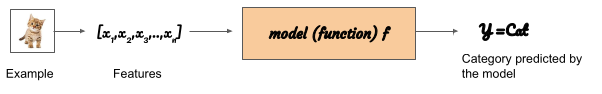
\includegraphics[width=0.6\linewidth]{imgs/15---classificazione-gatto}
    \caption{Esempio classificazione gatto}
    \label{fig:classificazione_gatto}
\end{figure}


\subsubsection{Regressione}
Al sistema viene chiesto di predirre un numero dati degli input.


\begin{figure}[H]
    \centering
    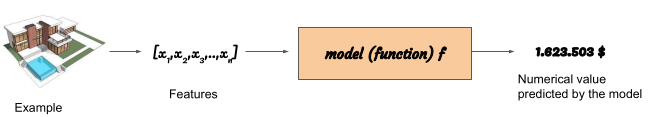
\includegraphics[width=0.6\linewidth]{imgs/16---regression}
    \caption{Esempio regressione}
    \label{fig:regressione}
\end{figure}


\subsubsection{Clustering}
Al sistema viene chiesto di ragruppare set di oggetti in modo che in un gruppo ci siano
oggetti simili tra loro rispetto agli altri gruppi.

\begin{figure}[H]
    \centering
    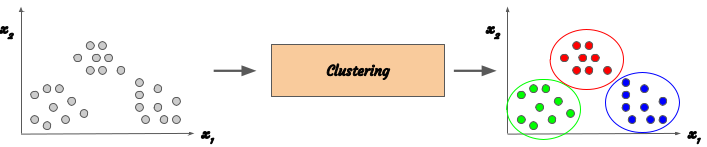
\includegraphics[width=0.6\linewidth]{imgs/17---clusetering}
    \caption{Esempio clustering}
    \label{fig:clustering}
\end{figure}



\subsubsection{Altre task}
\begin{itemize}
    \item transcription: data una immagine, descrivere con il testo
    \item machine translation
    \item anomaly detection
    \item imputation of missing value
    \item denoising
    \item density estimation
    \item synthesis
\end{itemize}

\subsection{Esperienza E}
L'esperienza è descritta da un dataset, solitamente di usa una matrice X
contenente nelle colonne tutte le features del data set(una features a colonna
, quindi ogni riga è un dato diverso).

\subsection{Labels}
Le etichette sono essenziali per fare task supervisionate, permettendo di misurare le
performance del sistema.

Possiamo assegnare ad ogni esempio una label che dice il valore corretto da predirre(Y).

\subsection{Modi per apprendere da esempi}
\begin{itemize}
    \item unsupervised learning
    \item supervised learning
    \item semi-supervised learning
    \item Reinforcement learning
\end{itemize}

Gli algoritmi non supervisionati vengono usati con dati senza label, l'algoritmo usando le features,
riesce a delineare delle classi all'interno dei dati.
Una task ricorrente nel unsupervised learning è il clustering.


Nel supervised learning, gli esempi includono un input e l'output desiderato(label), i modelli
più usati sono quello di regressione e classificazione.

semi-supervised learning, si hanno una parte di dati con le label e usando l'algoritmo si cerca di assegnare una label agli elatri elementi.



Reinforcement learning, l'esperienza non è rappresentata da un singolo dataset,
l'esperienza viene collezioanta da un "agent" che interagisce con l'ambiente, di modo
da aver un feedback loop tra il sistema e l'esperienza.

Vengono usati meccanismi di ricompensa e punizione.

\subsection{Modello di learning supervisionato}
Un modelo è uno strumento matematic che mappa l'input $X$ all'output $Y$
con la funzione $F$, dove $F$ è il modello.
I parametri si chiamano $w$.

Il modello è $y=F(X,w)$ e l'obbiettivo di ML è stimare i parametri $w$.

\subsubsection{Misura dell performance}
Una volta allenato un modello, si misura la performance(errori di classificazione
in task di classificazione o discostamento dal valore nei task di regressione).

Vogliamo sapere quato è bravo un modello a generallizzare il problema.
Per questo prima di applicare il modello, si separa il dataset in:
\begin{itemize}
    \item training
    \item test
\end{itemize}

\begin{figure}[H]
    \centering
    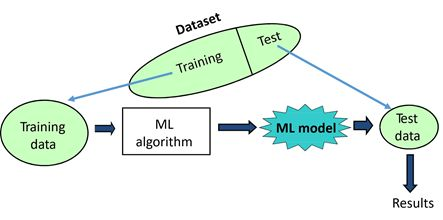
\includegraphics[width=0.5\linewidth]{imgs/18 - split}
    \caption{Split del dataset}
    \label{fig:split}
\end{figure}



\begin{figure}[H]
    \centering
    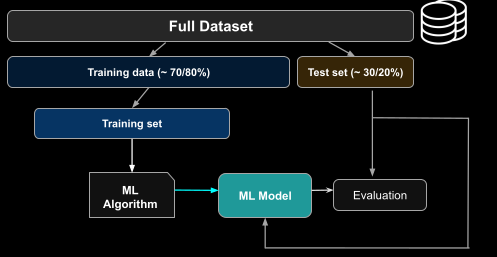
\includegraphics[width=0.5\linewidth]{imgs/19 - split2}
    \caption{Data splitting e ML}
    \label{fig:split_ML}
\end{figure}


\subsection{Loss function}
\begin{equation}
    J(w) = \frac{1}{2m}\sum_{i=1}^{m}(y_i-y_i^*)^2
\end{equation}
\begin{itemize}
    \item m è il numero di esempi
    \item $y^*$ è l'output del modello lineare
\end{itemize}
si cerca di minimizzare la loss usando delle w(parametri).

\subsubsection{Discesa del gradiente per minimizzare la loss(J)}

\begin{enumerate}
    \item abbiamo una $J(w_0,w_1)$
    \item vogliamo minimizzare J
    \item prendo una W random
    \item cerco W randomiche finchè non ottengo la J più piccola
\end{enumerate}

\begin{equation}
    W_j := \alpha\frac{d}{dW_j}J(W_0,W_1)
\end{equation}

$\alpha$ è il learning rate.

\begin{figure}[H]
    \centering
    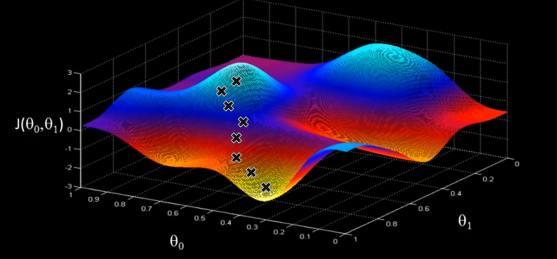
\includegraphics[width=0.5\linewidth]{imgs/discesa-gradiente}
    \caption{Discesa del gradiente}
    \label{fig:discesa_gradiente}
\end{figure}

\subsection{Discesa stocastica del gradiente(SDG)}
La discesa del gradiente è lunga e lenta perchè prende tutti i valori del
dataset, allora si usa La discesa del gradiente stocastica.

La SDG prende un'ostanza random nel training set ad ogni passo
per il calcolo del gradiente.
È più veloce.

Essendo randomica la natura del SGD, è meno regolare del gradiente normale
e migliora la discesa nella media in base alla "fortuna" del punto di
partenza.

\subsection{Regressione lineare}
Modello che fitta una linea retta.
\begin{equation}
    Y=W^{T}X
\end{equation}
Dove la $X$ è la matrice delle features e $Y$ è il vettore colonna che
contiene i target.

Calcola il gradiente cercando di ottimizzare al massimo la loss con
la linea retta.

\subsubsection{Problemi}
Avendo un modello polinomiale si può ottenere spesso un risultato migliore.

Se il data set è troppo piccolo, si tende ad andare in over fitting(il modello impara a
memoria i punti e con punti diversi va in crisi).


\subsubsection{Buonu dataset per buoni modelli}
Il modello impara dai dati $\Rightarrow$ i dati determiano la riuscita del modello.

Un buon dataset deve essere:
\begin{itemize}
    \item grande
    \item corretto
    \item consistente(esempi non contradditori)
    \item bilanciato(tutte le classi adeguatamente rappresentate)
\end{itemize}

\subsubsection{I.I.D}
Il training e il test devono essere generate da una distribuzione di probabilità.

\begin{itemize}
    \item Gli esempi nel dataset devono essere \textbf{indipendenti}
    \item il training e il test sono \textbf{identicamente distribuiti}(\textbf{I.I.D})
\end{itemize}


\subsubsection{Operfitting VS Underfitting}
\begin{figure}[H]
    \centering
    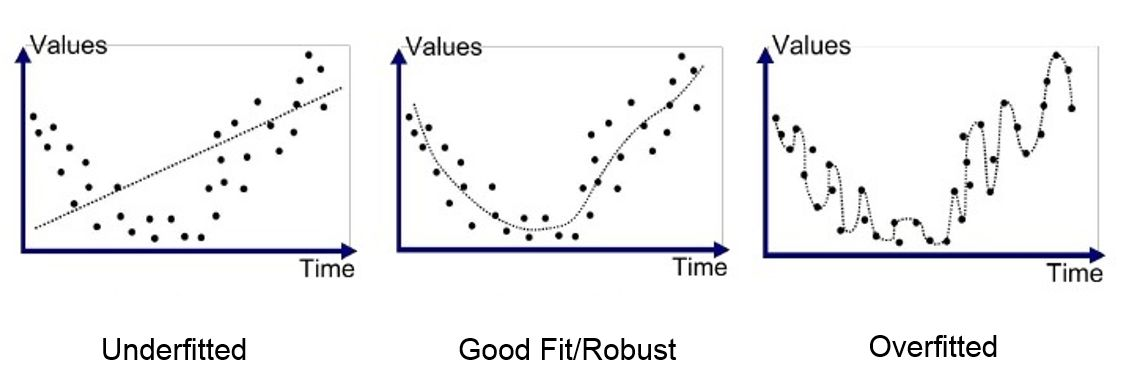
\includegraphics[width=0.6\linewidth]{imgs/underfitting_overfitting}
    \caption{Underfitting vs overfitting}
    \label{fig:under_over_fitting}
\end{figure}
Si va in \textbf{underfitting} quando un modello non riesce ad ottenere un errore
basso nel training set(probabile mancanza di dati).

Si va in \textbf{overfittin} quando gli errori nel test sono alti(probabilmente
il modello ha imparato a memoria il training).

Meglio avere un po di underfitting che overfitting, perchè nell'overfitting il modello
non è bravo a generalizzare.

\textbf{
    La chiave per è avere un errore in training basso ed
    avere il gap fra train e test basso.
}


\subsubsection{Capacità di un modello}

La capacità di un modello è l'abilità difittare una grande varietà
di funzioni.

Se ha poca capacità underfitta, se tanta capacità tende a overfittare.

Per controllare la capacità di apprendimento del modello, si usano
le \textbf{ipotesi dello spazio}(set di funzioni che il
modello può selezionare per la soluzione).


\begin{figure}[H]
    \centering
    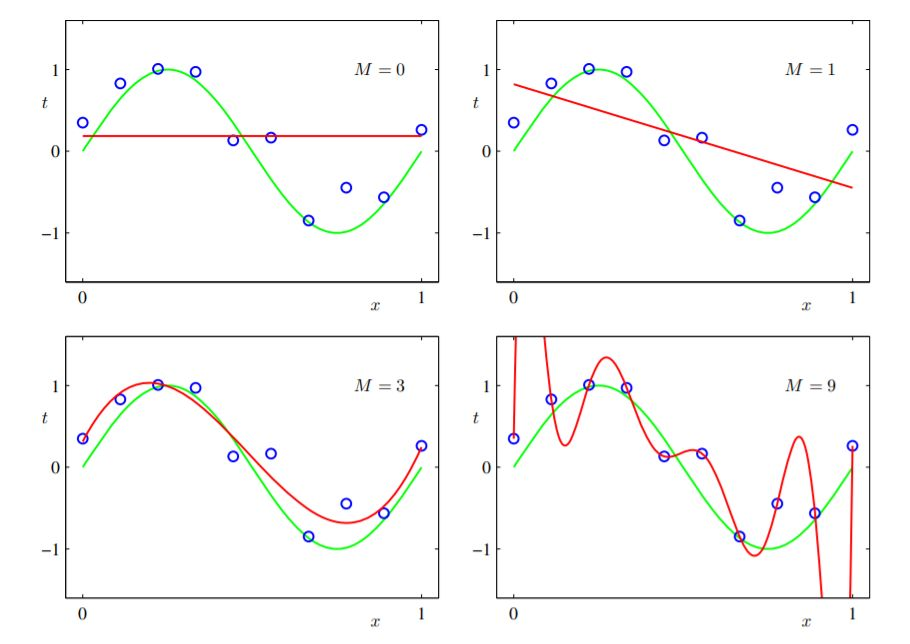
\includegraphics[width=0.6\linewidth]{imgs/ordine-polinomiale-under-over-fitting}
    \caption{Esempio di scelta del grado del polinomio}
    \label{fig:scelta_M}
\end{figure}

(regola a spanne)
Il numero di data points non dovrebbe essere meno di un x5/x10 del numero
di parametri del modello.

\subsubsection{Regolarizzazione}
Per ridurre l'overfitting, si aggiunge una penalità in termini di costo
alla funzione per scoraggiare l'overfitting.

Un aregola per la penalità semplice è la somma dei quadrati dei coefficenti:
\begin{equation}
    J(W) = \frac{1}{2m}\sum_{i=1}^{m}(Y_i-Y_i^*)^2 +
    \frac{\lambda}{2}\sum_{i=1}^{m}(W_J^2)
\end{equation}

Nel caso della regolarizzazione quadraica, prende il nome di \textbf{Ridge regression}
mentre nel neural networ si chiama \textbf{weight decay}.

\begin{figure}[H]
    \centering
    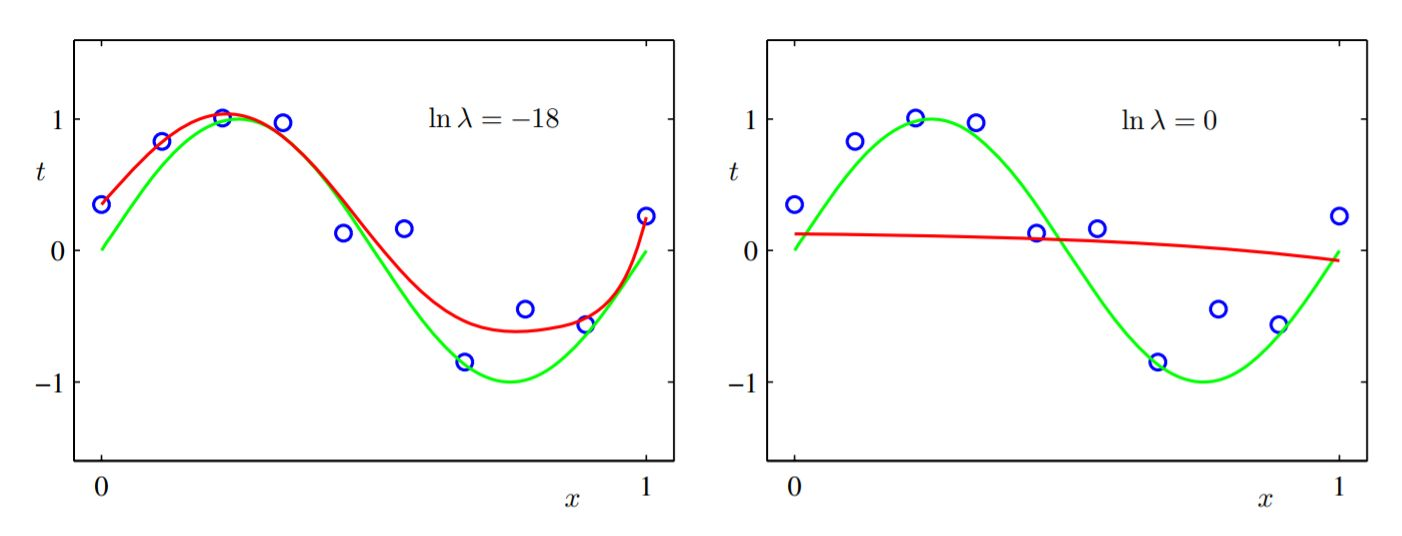
\includegraphics[width=0.5\linewidth]{imgs/esempio-lambda-regolarizzzazione}
    \caption{esempio regolarizzazione}
    \label{fig:esempio_lambda}
\end{figure}


\subsubsection{Validation set}
Il test set deve essere usato solo una volta per la vaalutazione del modello
 o modelli.

La vera division in train test e validation è:

\begin{figure}[H]
    \centering
    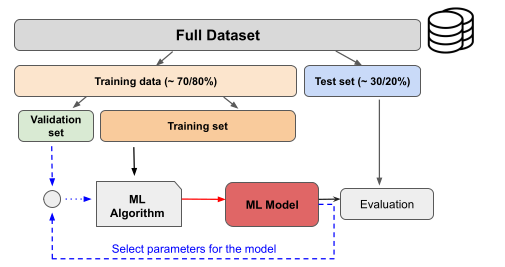
\includegraphics[width=0.65\linewidth]{imgs/train-test-validation}
    \caption{Vero train test validation}
    \label{fig:train_test_val}
\end{figure}
\begin{itemize}
    \item \textbf{training set}: dateset dove apprendere
    \item \textbf{validation set}: moddare i parametri del modello
    \item \textbf{test set}: MAI USARE, usare solo alla fine per la capacità
    di generalizzazione del modello
\end{itemize}

Ovviamente se il dataset in principio era bilanciato, ogni sotto insieme deve
essere bilanciato.













    \section{Classificazione}
Al sistema viene chiesto a quale categoria l'input appartiene.

Se il valore da predirre è un numero, si parla di una task di regressione,
se si vuole predirre un valore fra un numero di valori predefinito, si parla di
classificazione.

Esempi:
\begin{itemize}
    \item predirre un prezzo $\Rightarrow$ regressione
    \item predirre cane o gatto $\Rightarrow$ classificazione
    \item predirre cancro $\Rightarrow$ classficazione binaria
\end{itemize}


\subsection{Modello per la classificazione}
\subsubsection{Regressione logistica}
\begin{equation}
    h_W(X) = \frac{1}{1+e^{-W^{T}x}}
\end{equation}



La regressione logistica è un algoritmo di classificazione, stima la probabilità
che un istanza appartenga ad una classe (classificaione binaria).

La funzione è una sigmoide che da un output fra o e 1.

\begin{figure}[H]
    \centering
    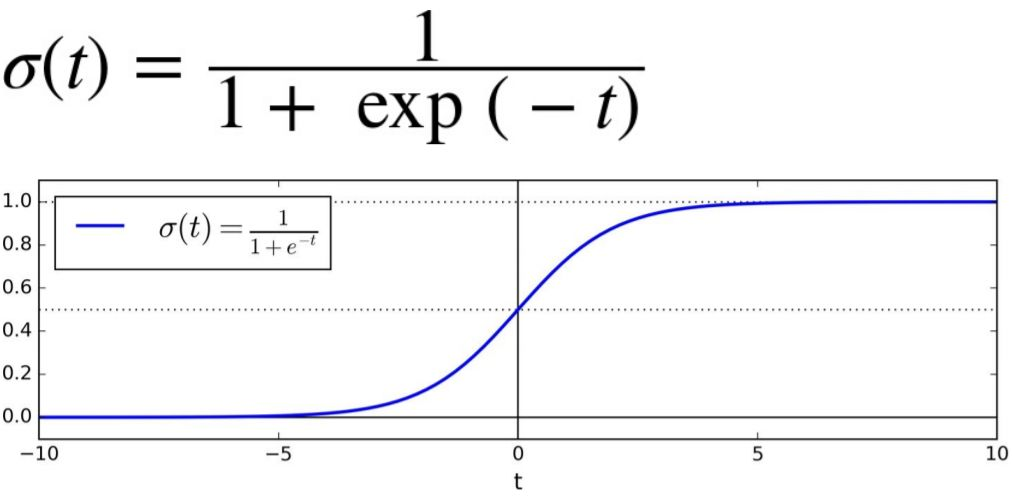
\includegraphics[width=0.4\linewidth]{imgs/sigmoide}
    \caption{Sigmoide}
    \label{fig:sigmoide}
\end{figure}

\subsubsection{Funzione logistica}
La regressione logistica calcola dei pesi per gli input + un termine bias.

Si si devono attribuire più label, si utilizzano tante classificazioni binarie.

\subsection{Classificazione multi-classe}
\subsubsection{One vs All}
Vengono allenate tante logistc classifier(binary), un classificatore per
ogni classe, poi si classifica in base alla probabilità dell oggetto per ogni classe.



\subsection{Dare un voto alle task di calssificazione}
\begin{itemize}
    \item matrice di confusione
    \item accuratezza
    \item precisione
    \item recall
    \item F-1
    \item curva di ROC
\end{itemize}

\subsubsection{Matrice di confusione}


\begin{figure}[H]
    \centering
    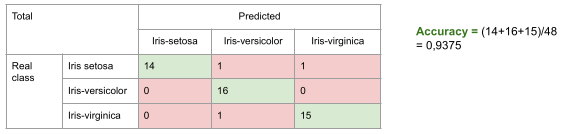
\includegraphics[width=0.5\linewidth]{imgs/matrice-di-confusione}
    \caption{matrice di confusione}
    \label{fig:conf_matrix}
\end{figure}

\subsubsection{Accuratezza}
Rapporto tra le predizioni corrette sul totale delle predizioni.(spesso si usa
la percentuale)


\textbf{Se il test set non è bilanciato, questo valore non ha nessun senso utile.}

\subsubsection{dataset non bilanciato}
Se il dataset non è bilanciato non devo vedere quante volte ci prendo sul totale
ma quante volte ci prendo sulla classe in analisi.

\subsubsection{Precisione}
Come l'accuratezza delle predizioni positive.

\begin{figure}[H]
    \centering
    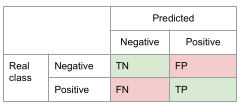
\includegraphics[width=0.2\linewidth]{imgs/precisione}
    \caption{Precisione}
    \label{fig:precisione}
\end{figure}


\begin{equation}
    Precisione = \frac{TP}{TP+FP}
\end{equation}


\subsubsection{Recall}
Conosciuta anceh come sensibilità o rateo di veri positivi.

È il rapporto di istanze positive che vengono correttamente trovate
dal classificatore.

\begin{equation}
    Recall = \frac{TP}{TP+FN}
\end{equation}

\subsubsection{F-1}
Misura armonica di precisione e recall,
tratta tutti i valori in maniera uguale,
attribuendo maggiore importanza ai valori bassi.

Un F1 alto è caratterizzato sia da recall alto che da precision alto!


\begin{equation}
    F_1 = \frac{2}
    {\frac{1}{Precision} +
    \frac{1}{Recall}}
\end{equation}


\subsubsection{Decision tree}
Modello ML simile ad un flowchart, le foglie sono le
classi(usabile sia in regression che classification).

Nel decision tree si usa il GINI.
\begin{equation}
    G_i = 1 - \sum_{k=1}^{n}p_{i,k}^2
\end{equation}

Si cerca d iscendere fino ad avere un gini = 0.

\subsubsection{CART}
CART(Classification and Regression Tree algorithm)
\begin{enumerate}
    \item dividi il training in 2 subsets usando una features k e una trashold $t_k$
    \item per prendere k e $t_k$ ci si basa sul subset più puro
    \item si ferma quando si raggiunge la profondità massima
\end{enumerate}

\begin{figure}[H]
    \centering
    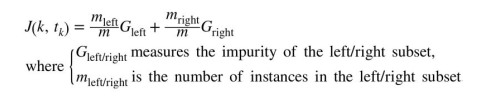
\includegraphics[width=0.7\linewidth]{imgs/cart}
    \caption{CART}
    \label{fig:CART}
\end{figure}

\subsubsection{Gini VS Entropia}
In ML, l'entropia è zero solo se l'istanza contiene una classe.

\begin{equation}
    H_i = - \sum_{k=1, P_{i,k}\neq 0}^{n}
    p_{i,k}\log(p_{i,k})
\end{equation}

Non ci sono tante differenze fra gini e entropia, solo che il gini essendo una sommatoria
è più veloce da calcolare e tende ad isolare la classe più frequente,
mentre l'entropia produce alberi più bilanciati.

\subsubsection{Regressione con alberi decisionali}
L'algoritmo splitta a scalini il tutto in mod oda avere tante istanze
di training vicine al possibile valore:
\begin{figure}[H]
    \centering
    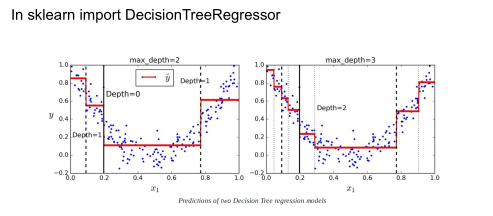
\includegraphics[width=0.5\linewidth]{imgs/decisiontreeregressor}
    \caption{DecisionTreeRegressor}
    \label{fig:DecisionTreeRegressor}
\end{figure}


Il CART funziona come prima però non cerca di splittare il
training set ma di minimizzare le impurità.

\subsubsection{Problemi: overfitting}
\begin{itemize}
    \item i decison tree fanno meno assunzioni rispetto al modello lineare
    \item se lasciato senza vincoli, va SUPER in over fitting
    \item l'albero è più libero come parametri, mentre la regressione lineare è
    più vincolata
\end{itemize}

\subsubsection{Soluzione: regolarizzazione}
Una soluzione è risurre i gradi di liberta dell'albero durante la fase di
training(regolarizzazione).
\begin{itemize}
    \item massima profondità
    \item numero minimo di campionimassimo numero di features per dividere i nodi
\end{itemize}

Metodologia del \textbf{pruning}, prima si fa il modello senza vincoli e poi si
applicano vincoli in base al caso.



Sensibili alla rotazione della matrice dei dati.
    \section{Frameworks for Big Data}

I sistemi RDBMS tradizionali sono comodi per fare input e output di dati
ma non sono ideali per l'analisi dei dati.

\subsection{Vincolati vs senza vincoli}
Un dataset vincolato ha una massima capacità di dati, mentre
quello non vincollato come lo streaming non ha un limite prestabilito.

\subsubsection{Ubounded dataset - dominio temporale}















































    \section{Ensamble learning}
Si fanno tante predizioni e poi si combinano.

\begin{figure}[H]
    \centering
    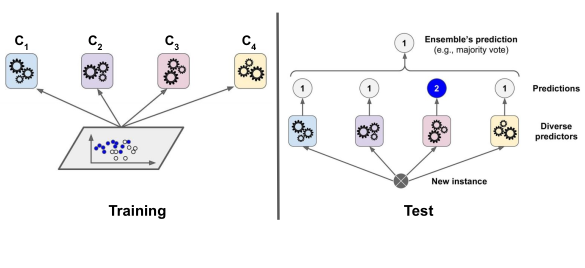
\includegraphics[width=0.8\linewidth]{imgs/ensemble-learning}
    \caption{Ensemble learning}
    \label{fig:Ensemble_learning}
\end{figure}

Se ho tanti classificatori, posso ripetere la classificazione su tatnti modelli diversi
con i corrispettivi errori(\textbf{indipendenti fra loro}).

Ho modo di aumentare la probabilità di prenderci se i modelli che uso
sono separati fra di loro, e le decisoni quindi non sono condizionate
dagli altri modelli.

\subsection{Bootstrap aggregating(Bagging)}
Se ho un solo dataset, porto ai modelli comunque lo stesso dataset con gli stessi
errori comuni, uso la tecnica di \textbf{bootstrapping} dove porziono il dataset
in sotto sezioni e assegno diverse sezioni a diversi modelli,
cosi da eliminare anche i problemi legati ai dati simili.

\subsection{Random forest}
È un mmodello bagging dove fa l'aggregazioni di alberi decisionali.

\subsection{Hard voting classifier}
Usare algoritmi diversi con classificatori diversi e poi fare un hard voting
\textbf{codice di pag 22 cap 13 figo}

\subsection{Boosting}
Simile al bootstrapping ma fatto in maniera sequenziale(l'output di uno è l'input del successivo).

Ogni predizione cerca di correggere la precedente.

\subsubsection{AdaBoost}
\begin{itemize}
    \item per correggere il predecessore, presta attenzione alle istanze del training
    che il predecessore ha underfittato
    \item il nuovo "predittore" si concentra di più sul hard case(adaptive)
    \begin{enumerate}
        \item La prima predizione è treinata e usata per fare predizioni sul training
        \item I pesi di missclassification vegono incrementati
        \item la seconda classificazione usa i pesi aggiornati
        \item Ad ogni classificatore viene assegnato un peso
        \item Dopo che ogni "predicter" ha finito il train, viene fatta unapredizone come nel
        bagging, tranne per il fatto che le predizioni hanno un peso.
    \end{enumerate}
\end{itemize}

\begin{figure}[H]
    \centering
    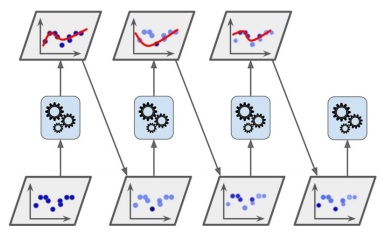
\includegraphics[width=0.3\linewidth]{imgs/ada-boosting}
    \caption{AdaBoost}
    \label{fig:AdaBoost}
\end{figure}

\subsubsection{Algoritmo di AdaBoost}
Ongi istanza ha un peso w,
inizialemnte settato a $\frac{1}{m}$,
dove m è il numero delle osservazioni.
Per ogni predicotr J, viene calcolato un peso di error-rate $r_J$.

\begin{equation}
    r_J = \frac{
        \sum_{i=1, \hat{y}_j^{(i)}\neq y^{(i)}}^{m} w^{(i)})
    }{
        \sum_{i=1}^{m} w^{(i)})
    }
\end{equation}

Poi viene calcolato il peso $\alpha_J$ in base al learningn rate $\eta$.

Più un predittore è accurato e maggiore sarà il suo peso:
\begin{equation}
    \alpha_J = \eta\log\frac{1-r_J}{r_J}
\end{equation}

Se prova a indovinare a caso ($50\%$) avrà valore vicino a 0, se sbagli il più
delle volte, sarà negativo il suo valore.


Dopo di chè i pesi delle istanze vengon aggiornati con:
\begin{equation}
    w^{(i)}
    \begin{cases}
        w^{(i)} \Rightarrow if \hat{y_j}=y(i) \\
        w^{(i)} \exp(\alpha_j) \Rightarrow if \hat{y_j}\neq y(i)
    \end{cases}
\end{equation}

Dopo aver aggiornato tutti i pesi, adaBoost computa la predizione usando i pesi.

La classe predetta è quella che prende la magioranza di voti pesati.

\subsubsection{Gradient Boosting}
La chiave del GB è la additività dei modelli, si puo arrivare ad avere
un imparatore finale:
\begin{equation*}
    F_L=f_0(x) + \dots + f_{L-1}(x)
\end{equation*}

dove la L è il numero di learner che si usano ed f0 è il primo learner che apprende
dal dataset, gli altri learner dopo di lui cercano di migliorare il risultato
riducendo la loss function.

Ogni learner prende il nome di epoch, e durante ogni epoch si cerca di ridurre la
loss e non di aumentare le istanze(come fa adaBoost).





































    \section{Design principles for ML}


\begin{figure}[H]
    \centering
    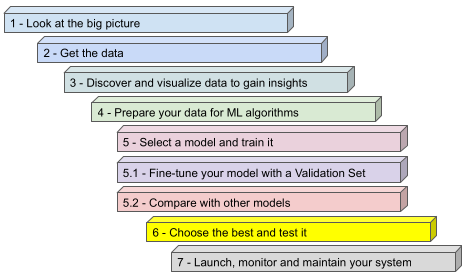
\includegraphics[width=0.6\linewidth]{imgs/design-principles-for-ml}
    \caption{Design principles for ML}
    \label{fig:Design_principles}
\end{figure}

\subsection{Look at the big picture}
\begin{enumerate}
    \item Definire gli obbiettivi in termini di business
    \item come verrà usata la mia soluzione?
    \item Come voglio risolvere il problema? task supervisionata o non? regressione o classificazioen?
    \item Cme dovrebbe essere misurata la performance? la performance si allinea agli
    obbiettivi del business? quale è la performance minima da ottenere per il business?
\end{enumerate}


\subsection{Get the data}
\begin{enumerate}
    \item quali dati e wuanti mi servono
    \item converti i dati in un formato facile da manipolare senza modificare i dati
    \item dati sensibili eliminati
    \item controlla la dimensione e la grandezza dei dati
    \item crea un test set e mettilo da parte(usalo solo per il check finale di generalizazione)
\end{enumerate}

\subsection{Explore the data}
\begin{enumerate}
    \item studia gli attributi del tuo dataset
    \begin{enumerate}
        \item tipo(categorico o numerico)
        \item bounded/unbounded
        \item testo o struttura
        \item percentuale di valori mancanti
        \item rumore e tipo di rumore
        \item vedere se gli attributi sono utili per il test
        \item distribuzione dei dati
    \end{enumerate}
    \item per i task supervisionati, identifica le label (Y)
    \item visualizza i dati
    \item studia la correlazione tra attributi
\end{enumerate}

\subsection{Prepare your data for the ML algorithms}
\begin{enumerate}
    \item Pulizia dei dati
    \begin{enumerate}
        \item ripara o rimuovi gli outliners(optional)
        \item riempi i dati mancanti
    \end{enumerate}
    \item selezione delle features(optional)
    \item ingegnerizzazione delle features
    \begin{enumerate}
        \item rendi featire continue discrete
        \item aggiungi trasformazioni comode delle features come il log
        \item aggrega features in nuove più promettenti
    \end{enumerate}
    \item features scaling(normalizzare e standardizzare le features)
\end{enumerate}

\subsubsection{Features scaling}
Uno delle fasi di pre processamento più importanti, permette di rendere la discesa del gradiente
più rapida.
Avendo le features tutte su una scala uguale, anche se il gradiente scegli
il punto di partenza a caso, non ho dei range di varizione ampissimi.
Se ho le features non scalate correttamente posso avere dei casi estrememaente lenti.


\begin{figure}[H]
    \centering
    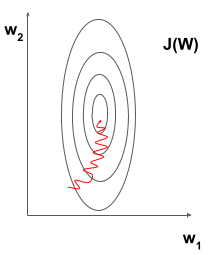
\includegraphics[width=0.3\linewidth]{imgs/featues-scaling-1}
    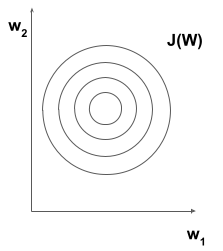
\includegraphics[width=0.3\linewidth]{imgs/scaling-2}
    \caption{Features scaling}
    \label{fig:scaling1}
\end{figure}

Cosi avremo una discesa del gradiente più regolare e meno suscettibile alle dimensioni
delle features.

\subsection{Feature scaling types}
\subsubsection{Min-Max normalizing}
\begin{equation}
    x' = \frac{x - min(x)}{max(x)-min(x)}
\end{equation}


\subsubsection{Mean normalizing}
\begin{equation}
    x'=\frac{x - average(x)}{max(x)-min(x)}
\end{equation}
\subsubsection{Standardizzation(or Z-score)}
\begin{equation}
    x'=\frac{x-average(x)}{\sigma}
\end{equation}
Dove sigma è la deviazion standard.

Ricordati che il preprocessing lo fai sul training, una volta ottenuto il tuo modello
per testarlo sul test, applica la standardizzation sul test e poi dallo al modello.

\subsection{Features selection}
\begin{itemize}
    \item alcune featires sono inutili
    \item se ho meno ridondanza, ho meno overfitting
    \item risualtato migliore
    \item meno tempo di training
\end{itemize}

\subsubsection{Univariate feature selection with chi2 test}
scegli le migliori featues usando chi2.
Questo risultato(chi2) può essere usato per selezionare le features.

Questo punteggio può essere usato per vedere quali features usare
in base al malore più alto del chi2 test, che deve avere solo valori positivi.

Il chi2 da un voto più alto alle features che sono più dipendenti con le altre
e un voto più basso alle features più indipendenti.


\subsubsection{Feature selection with Mutual information}
La mutua informazione(MI) è un numero alto se fra due variabili random
la dipendenza è alta.

Valore alto significa grande dipendenza.



Chi2 stima il grado di dipendenza lineare fra due variabili random, invece MI,
cattura ogni informazione inerente alla dipendenza statistica,
ma non essendo parametrizzabile, richiede più esempi per maggior precisione.

\subsection{Assunzioni sui dati}
\begin{itemize}
    \item un modello è una versione semplice del'osservazione, il semplificata significa che
    il modello scarta dettagli superflui che non sa generalizzare.
    Comunque, per decidere che dati scartare, devo fare \textbf{assunzioni}.
    \item Senza fare assunzioni sui dati, non c'è motivo di preferire un modello ad
    un'altro(\textbf{teoria del no più pranzo gratis})
    \begin{itemize}
        \item nessun modello funziona meglio a prescindere
        \item per capire quale modello è meglio faccio le prove e li valuto
        \item in alternativa alle prove, posso ragionare e fare assunzioni(linea guida generalissima)
        \begin{itemize}
            \item task semplici $\Rightarrow$ modello lineare con vari gradi di regolarizzazione
            \item task difficili $\Rightarrow$ reti neurali
        \end{itemize}
        \item attenzion al numer odi features rispetto al numero dei dati
    \end{itemize}
\end{itemize}

Un idea buona è di testare tanti modelli sui dati, ma questo porta ad un error
stocastico dei modelli e la divisione del dataset in test e train in maniera randomica.

Una soluzione potente è far fare tanti giri ad ogni signolo modello cosi  ta eliminare
il più possibile gli errori di natira stocastica.

minimo 10 giri suggeriti dal prof!

Una volta trovato l'algoritmo che fa meglio quel lavoro, si può fare
il \textbf{fine-tuning} degli hyper-parameters del modello.

\subsubsection{Come miglirare gli hyper-parameters}

Due modi principali:
\begin{itemize}
    \item Grid-search
    \begin{itemize}
        \item provare le combinaioni di preset e annotarsi i risultati
        \item quando ho finito le combinazioni, il modello viene fatto con le combinazioni di parametri migliori
        \item Il tempo pper valutare questo cresce in maniera esponenziale con l'aggiunta di parametri
    \end{itemize}
    \item random search
    \begin{itemize}
        \item si va a caso e si annotano i risulati con il tuning randomico fatto
        \item funziona con pochi dati
        \item è pprovato che il random è meglio empiricamente del grid
        \item se il dataset è grande, meglio usare in combo il random e il grid
    \end{itemize}
\end{itemize}


\subsection{K-fold cross-validation}
Se ho un data set piccolo uso questo trick,
divido il dataset in porzioni e a turno le do in pasto al modello(sempre per il discorso di fargli fare tanti giri).

\begin{figure}[H]
    \centering
    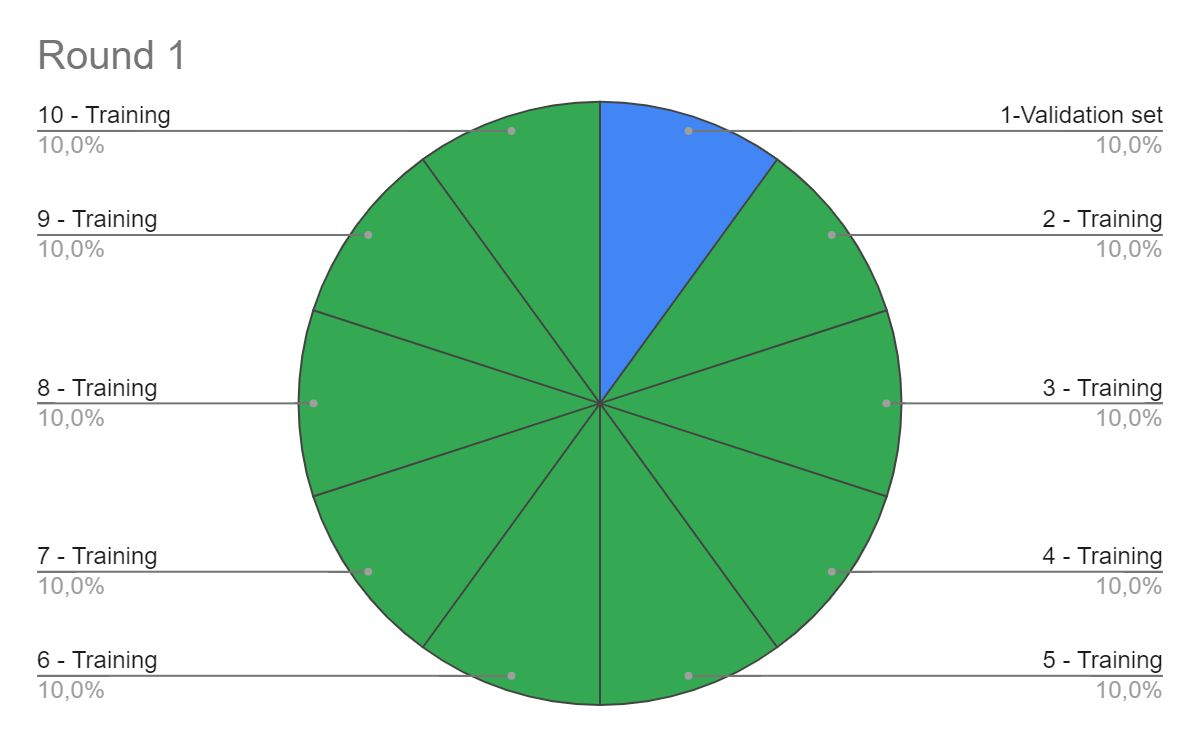
\includegraphics[width=0.6\linewidth]{imgs/k-fold}
    \caption{K-fold}
    \label{fig:kold}
\end{figure}


La cross validation permette di torvare oltre alla stima del modello,
ti permette acneh di capire quanto un modello è preciso.(tipo deviazione standard e altri)


\subsection{Riassunto della pipeline}
\begin{enumerate}
    \item Dividi il dataset in 80 training e 20 test
    \item applica il features scaling
    \item dal training estrai un 10 come validation(usa il validation per i test e il fine-tuning, se hai pochi dati usa il k-fold)
    \item crea un grid o un random search sui possibili parametri e valuta il modello con il validation set
    \item quando ha iun buon risultato, valuta il modello sul test setper vedere la generalizzazione
\end{enumerate}

\section{Unsupervised Learning}

I dati non hanno una label,
alcune task:
\begin{itemize}
    \item clustering
    \item dimensionality reduction
    \item anomaly detection
\end{itemize}

\subsection{Clustering}
Al sistema viene chiesto di raggruppare set di oggetti in gruppi(cluster), di modo
che gli oggetti di un gruppo siano parecchio simili.

Usato per trovare proprietà nascoste o irregolarità.

Anche il clustering è un problema di ottimizzazione, cerchiamo di raggruppare oggetti
in gruppi, entrano in gioco concetti come \textbf{variabilità(c)} e \textbf{dissimilarità}.

\begin{equation}
    variability(c_i) = \sum_{e\in c_i} distance(mean(c_i), e) ^2
\end{equation}

\begin{equation}
    dissimilarity(c) = \sum_{c_i\in c} variability(c_i)
\end{equation}

Per ottimizzare devo trovare dei cluster che minimizzino la dissimilarità con un numero
di cluster che decidiamo a priori(usare un cluster avrebbe dissimilarità bassa ma  non serve a
nulla).

I due metodi principali per il clustering sono: hierarchical clustering e K-Means.


\subsubsection{Hierarchical clustering(agglomerative clustering)}

\begin{enumerate}
    \item inizio con dare un cluster ad ogni oggetto(quindi ho un cluster per ogni oggetto e ogni claster contiene un oggetto)
    \item trova la coppia di cluster più simili e fai un merge
    \item ripeti fino ad ottenere un cluster di N item
\end{enumerate}

Trovare le coppie simili prende il nome di linking,
può essere singolo(semplice) o completo:
\begin{figure}[H]
    \centering
    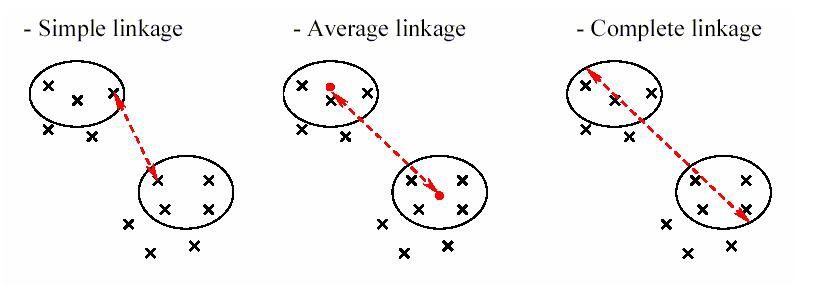
\includegraphics[width=0.6\linewidth]{imgs/linkag}
    \caption{Linkage}
    \label{fig:Linkage}
\end{figure}
\begin{itemize}
    \item simple linkage: la distanza fra cluster è tra i membri più vicini dei due cluster
    \item complete linkage: vede la distanza come la distanza massima possibile fra i due cluster
\end{itemize}


\begin{figure}[H]
    \centering
    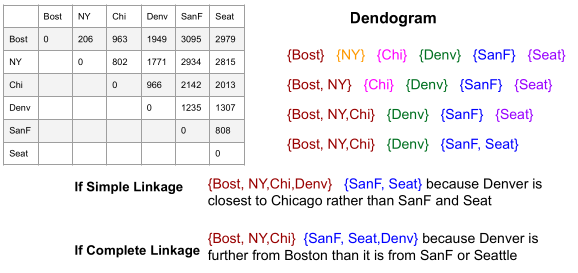
\includegraphics[width=0.6\linewidth]{imgs/esempio-clustering}
    \caption{Esempio clustering}
    \label{fig:Esempio-clustering}
\end{figure}


Nei cluster gerarchici:
\begin{itemize}
    \item il criterio di linking e deterministico(no random)
    \item il dendogramma è facilmete spiegabile
    \item è un algoritmo greedy
    \item è flessibile(cambia cirteri per differenti risultati)
    \item lento( complessità $O(N^3)$)
\end{itemize}


\subsubsection{K-Means}
\begin{itemize}
    \item Serve un algoritmo greedy più veloce
    \item k è il numero dei cluster che voglio
    \begin{enumerate}
        \item scegli un numero radom di centroidi k
        \item while true:
        \begin{enumerate}
            \item crea k cluster assegnando ogni esempio al centoride più vicino
            \item computa k nuovi centroidi facendo la media in ogni cluster
            \item se i centroidi non cambiano
            \begin{enumerate}
                \item fermati
            \end{enumerate}
        \end{enumerate}
    \end{enumerate}
\end{itemize}
\begin{figure}[H]
    \centering
    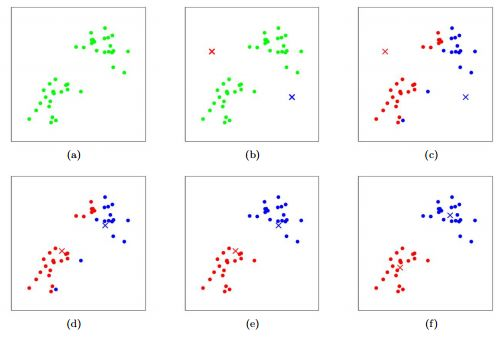
\includegraphics[width=0.8\linewidth]{imgs/k-means}
    \caption{k-means}
    \label{fig:k-means}
\end{figure}


\subsection{La maledizione della dimensionalità}
È il problema che esce quando si danno ai modelli dati con multidimensionali.

Se si aggiungono tante features da prendere in considerazione, si possono separare
le classi in analisi ma lo spazio diventa enorme, se si usano troppe features,
si rischia di ottenere una separazione per ogni elemento del sistema.

Con l'aumento della dimensionalità lo spazio cresce e i daati saranno sempre più
sparsi.

\begin{figure}[H]
    \centering
    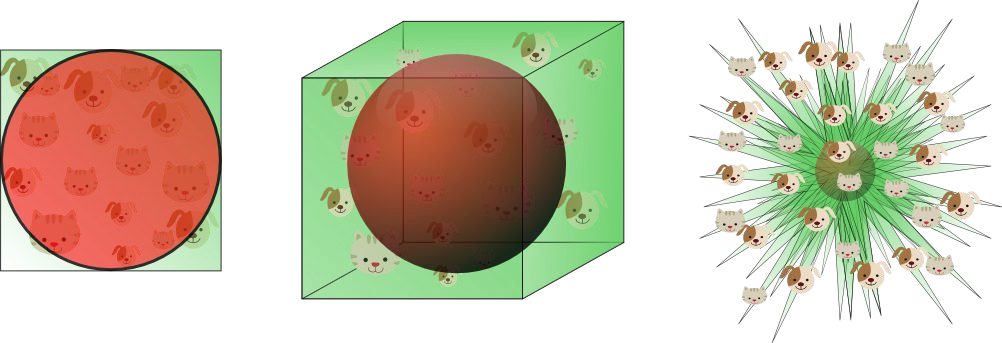
\includegraphics[width=0.6\linewidth]{imgs/curse-of-dimensionality}
    \caption{curse of dimensionality}
    \label{fig:curse_of_dimensionality}
\end{figure}
La quantità di dati richiesta da lproblema aumenta esponenzialmente con l'aumentare
della dimensionalità.

\subsection{Riduzione della dimensionalità}
Nei casi del mondo reale, i dati non sono sparsi nelle dimensioni in maniera uniforme,
alcune dimensioni sono costanti ecc.
La maggior parte delle istanze giace in un numero ristretto di dimensioni(o li vicino).


\subsubsection{Principal Component Analysis(PCA)}

PCA è l'algoritmo per la riduzione della dimensionalità più popolare.

\begin{itemize}
    \item identifica l'iperpiano che giace più vicino ai dati e li proietta su se stesso
    \item Per proiettare i dati su un iperpiano a dimensionalità minore, biogna trovare l'iperpiano giusto
    \begin{itemize}
        \item il miglio iperpiano è quello che conserva più dati
    \end{itemize}
\end{itemize}

\begin{figure}[H]
    \centering
    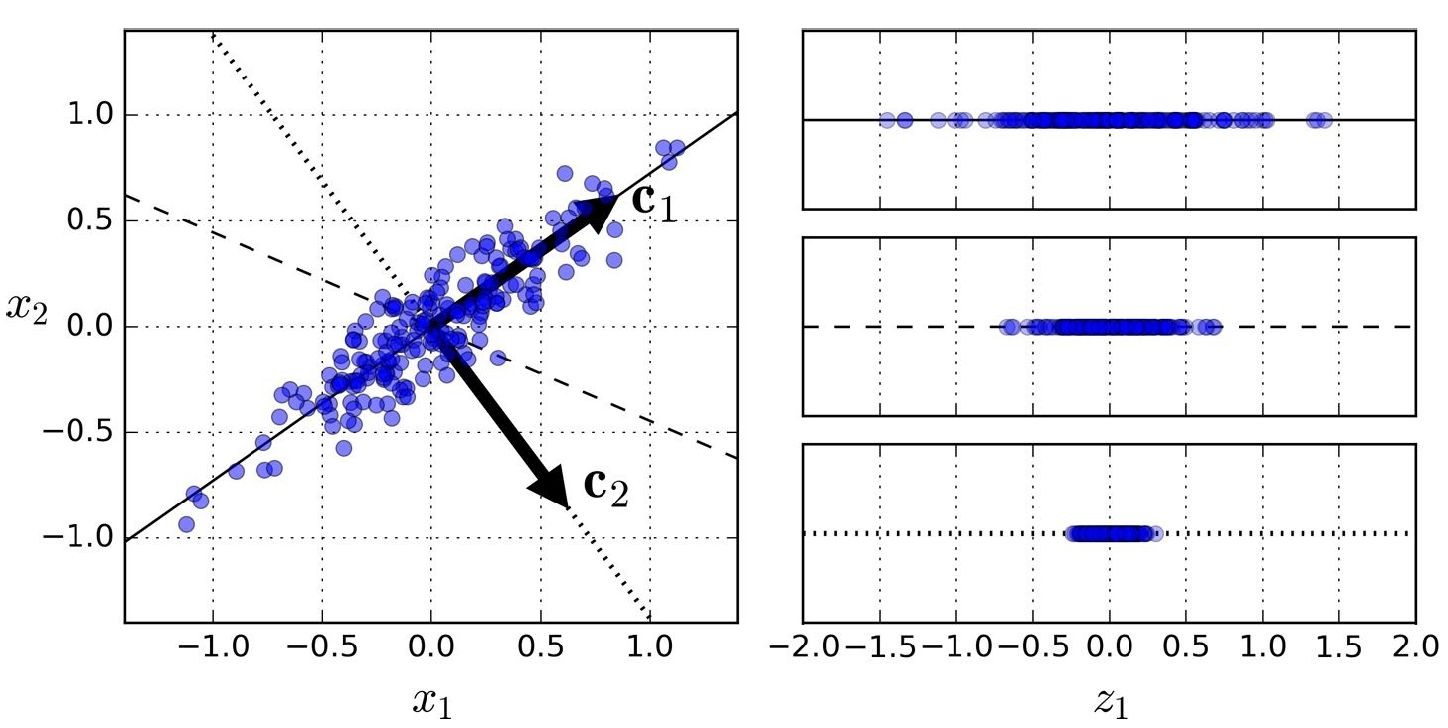
\includegraphics[width=0.5\linewidth]{imgs/pca}
    \caption{PCA}
    \label{fig:PCA}
\end{figure}
PCA identifica l'asse che prende il maggior numero di variazioni(come nell'esempio),
in base a che dimensione vuoi raggiungere, calcola anche il secondo/terno asse ecc.
Se per esempio vuoi ridure a tre assi, ti troverà i tre assi dove collassano più dati.


L'iesimo asse è chiamato l'iesimo componente principale.

Un avolta identificati componenti principali, puoi ridurre le dimensioni.

\subsubsection{t-SNE}
t-distributed Stochastic Neighbor Embedding(t-SNE) è una tecnica di riduzione
dimensionale non lineare.

È lo stato dell'arte per gli algoritmo di riduzione di dimensioni per la data
visualizzation.


Modella ogni oggetto con tante dimensioni in modo che gli oggetti simili sono
modellati da punti vicini e oggetti non simili con punti lontani


\begin{itemize}
    \item SNE comincia con il convertire le distanze euclidee multi-dimensionali fra
    i dati in probabilità condizionali che rappresentano le similitudini.
    \item t-SNE costruisce una distribuzione di probabilità sulle coppie di oggetti con tante
    dimensioni di modo che oggetti simili abbiano una alt probabilità mentre gli oggetti
    meno simili probabilità minore
    \item t-SNE definisce una distribuzione di probabilità sui punti nella mappa a meno dimensioni
    e minimizza la Kullback-leibler divergence(KL-divergence) tra le due distribuzioni usando
    la discesa del gradiente.
    \item genera una spazio random e ci mette i dati randomicamente
    \item poi minimizza la discesa KL del gradiente in modo da preservare la vera distanza
    fra gli oggetti.
\end{itemize}



\subsubsection{recap t-SNE vs PCA}
\begin{itemize}
    \item t-SNE è iterativo non come PCA, non puoi applicarlo ad unaltro dataset come se niente fosse
    Con PCA una volta ottenuta la prima riduzione, si puo riapplicare ad altri dati
    \item PCA crea un sub spazio di quello originale che nel ML è una features importante.

    \item t-SNE è sconsigliato per il ML perchè crea uno spazio artificiale
    dove le features legate alla spazio possono essere meno informative
\end{itemize}
























    \section{An introduction to
Neural Networks}

\subsection{Deep neural networks}
Il termine deep learning si rifà al training di differenti tipi di reti neurali caratterizzate
da diversi layer di neuroni(deep).

Alcuni esempi:
\begin{itemize}
    \item Multi-layer Perceptron with several hidden layers
    \item Convolutional Neural Networks (CNN)
    \item Recurrent Neural Networks (RNN)
    \item Auto-encoder for unsupervised learning
    \item Graph Neural Network (GNN)
    \item Graph Convolutional Network (GCN)
    \item transformers and Attention Models
    \item altri
\end{itemize}

\subsection{Neurone artificiale}

\begin{figure}[H]
    \centering
    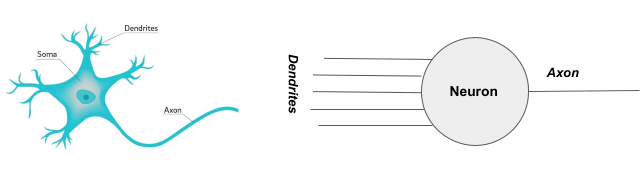
\includegraphics[width=0.5\linewidth]{imgs/neurone-artificale}
    \caption{Neurone artificiale}
    \label{fig:Neurone_artificiale}
\end{figure}

Dove sui dentriti si posizionano le features utili al modello.

Vengono applicati dei pesi e si fa una somma pesata per decidere il risultato.

Manca il bias(intercetta).
\begin{figure}[H]
    \centering
    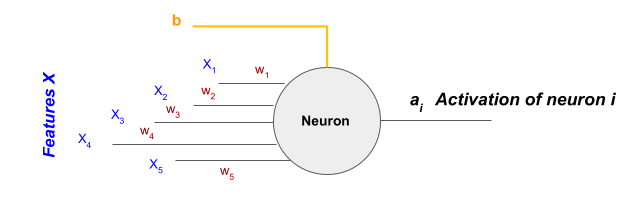
\includegraphics[width=0.5\linewidth]{imgs/neurone}
    \caption{neurone}
    \label{fig:neurone}
\end{figure}

Doev l'attivazione dipende da : $W^{TX+b}$

Fino ad ora molto simile ad una regressione lineare.

Possiamo cambiare la funzione di attivazione!!!

\begin{itemize}
    \item Un neurone artificiale è una funzione che mappa un vettore di features in input
    in uno scalare in output con un vettore di pesi e una funzione
    \item gli input sono i dendriti
    \item il valore scalare dell'output rappresenta l'attivazione del neurone
    \item il neurone riceve gli input pesati, computa l'output secondo la funzione di attivazione
\end{itemize}

\begin{figure}[H]
    \centering
    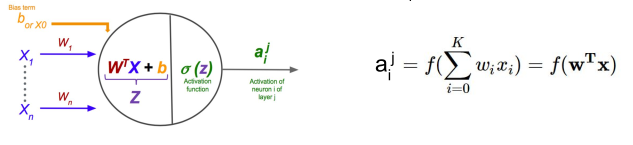
\includegraphics[width=0.8\linewidth]{imgs/neurone2}
    \caption{Funzionamento neurone}
    \label{fig:funzionamento_neurone}
\end{figure}

\subsubsection{Funzione di attivazione}
La funzione f del disegno qui sopra si chiama funzione di attivazione e genera
una relazion non lineare fra input e output.

Ci sono diverse funzioni di attivazione, la più comune è la sigmoide:
\begin{figure}[H]
    \centering
    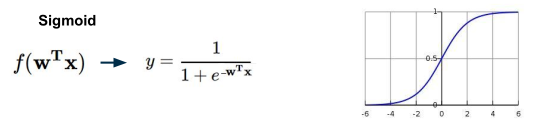
\includegraphics[width=0.7\linewidth]{imgs/sigmoide2}
    \caption{sigmoide}
    \label{fig:sigmoide2}
\end{figure}


\subsubsection{Un layer}
\begin{figure}[H]
    \centering
    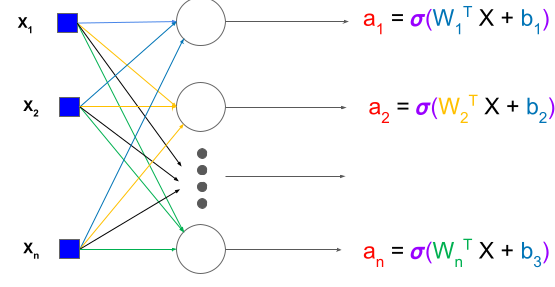
\includegraphics[width=0.7\linewidth]{imgs/layer}
    \caption{layer}
    \label{fig:layer}
\end{figure}


\subsection{Artificial Neural Network(ANN)}
I nodi di uno stattesso layer non counicano tra loro.

Ogni neurone si un layer è collegato a quello del layer successivo e precedente.

\begin{figure}[H]
    \centering
    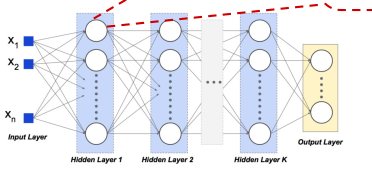
\includegraphics[width=0.6\linewidth]{imgs/ann}
    \caption{ANN}
    \label{fig:ANN}
\end{figure}


Ogni connessione fra neuroni è pesata!!

I pesi sono inizializzati ranodmicamente e l'obbiettivo della rete
durante il training è di imparare i pesi!!

\subsection{Layer di output}
La strutttura di questo laer dipende dal tipo di task.

Il vettore delle Y nel data set deve essere formattato a seconda di questo layer.

\begin{itemize}
    \item regresssione: usimao un neurone per predirre un valore(fuzione di attivazione probabilemte lineare)
    \item classificazione binaria: possimao finire con un neurone che usa una sigmoide(ci sono tanti altri modi)
    \item clssificazione multi classe o multi label: avremmo tanti nodi finali quante le classi(ogni neurone rappresenta una classe)
\end{itemize}


\subsection{Esempi}
\begin{figure}[H]
    \centering
    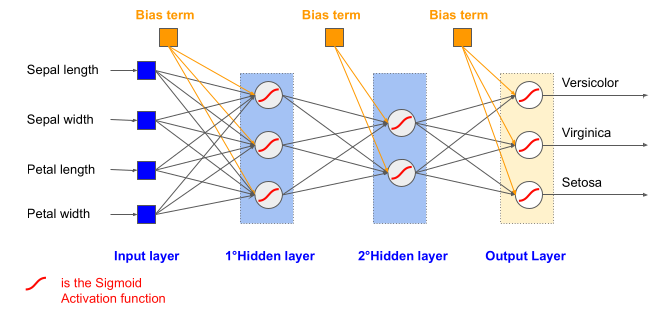
\includegraphics[width=0.8\linewidth]{imgs/iris}
    \caption{iris}
    \label{fig:iris}
\end{figure}
\begin{figure}[H]
    \centering
    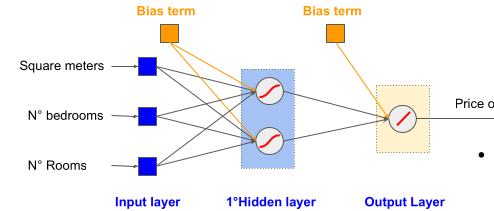
\includegraphics[width=0.8\linewidth]{imgs/case}
    \caption{case}
    \label{fig:case}
\end{figure}

\subsection{Funzioni di attivazione}

\begin{figure}[H]
    \centering
    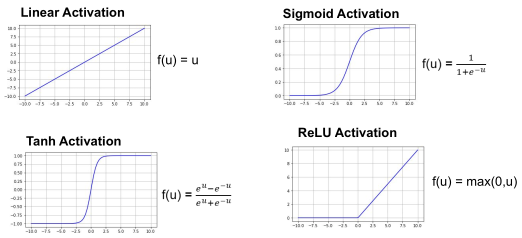
\includegraphics[width=0.8\linewidth]{imgs/funzioni_attivazione}
    \caption{funzioni di attivazione}
    \label{fig:funzioni_attivazione}
\end{figure}

\subsection{Rappresentazione latente}
La rappresentazion latente è quella fra 'ultimo layer nascosto
e il layer di output.

La responsabiltà di fare un task di classificazione o di regressione dipende dal come
viene fatto l'ultimo layer(quello di output).

\subsubsection{Softmax output(solo per la classificazione)}
\begin{figure}[H]
    \centering
    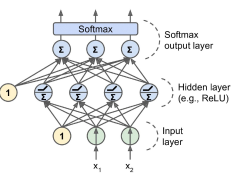
\includegraphics[width=0.5\linewidth]{imgs/softmax}
    \caption{softmax}
    \label{fig:softmax}
\end{figure}

Quando si fa una task di classificazione con multi classe, si può usare un softmax.

Si possono rimpiazzare le indiviuali funzioni del layer che classifica
con una softmax, loutput di ogni neurone (ultimo strato) corrisponde alla
probabilità di appartenere ad una classe.

La softmax è una generalizzazione di unaregressione lineare per supportare
tante classi direttamante senza dover fare una multi classificazione binaria.

La probabilità che un oggetto appartenga alla classe k è:
\begin{equation}
    \vec{p_k} = \sigma(S(X))_k =
    \frac{\exp(s_x(x))}{\sum_{j=1}^{k} \exp(s_j(x))}
\end{equation}

La softmax predice la classe con la maggior probabilità.

\subsection{Reti neurali: ottimizzazione}
\subsubsection{Funzioni di loss}
\begin{figure}[H]
    \centering
    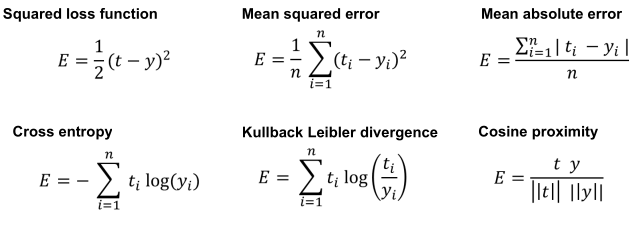
\includegraphics[width=0.8\linewidth]{imgs/funzioni-di-loss}
    \caption{funzioni di loss}
    \label{fig:funzioni_di_loss}
\end{figure}

\begin{itemize}
    \item task di regressione
    \begin{itemize}
        \item mean squared error loss
        \item mean absolute error loss
    \end{itemize}
    \item task di classificazione binaria
    \begin{itemize}
        \item binary cross-entropy
    \end{itemize}
    \item task classificazione multi-classe
    \begin{itemize}
        \item multi-class cross-entropy loss
        \item Kullback Leibler Divergence Loss
    \end{itemize}
\end{itemize}


\subsection{Allenanod un ANN: algortimi di backpropagation}

\begin{enumerate}
    \item inizializzo un ANN con pesi random
    \item propago ogni esempio nella rete dal input layer fino al layer di
    output e ottengo una predizione
    \item poi calcolo l'errore della predizione(differenza tra vero e predetto)
    \item misuro l'errore e provo a risurre l'errore aggiornando i pesi,
    propago l'errore indietro fino all'input
\end{enumerate}

\subsubsection{Backpropagation}
\begin{itemize}
    \item l'errore viene propagato fino all'input per aggiornare i pesi
    \item per sapere come aggioranre i pesi, dobbiamo fare il gradiente
    \item quindi si fa il gradiente per ogni layer partendo dall'output fino ad arrivare
    all'input
\end{itemize}

Si fa una discesa del gradiente per ridurre l'errore.

Il nuovo peso assume questo valore:
\begin{figure}[H]
    \centering
    \includegraphics[width=0.8\linewidth]{imgs/discesa-del-gradiente-ann}
    \caption{discesa del gradiente ANN}
    \label{fig:discesa_del_gradiente_ANN}
\end{figure}
\begin{figure}[H]
    \centering
    \includegraphics[width=0.8\linewidth]{imgs/discesa-del-gradiente-ann2}
    \caption{discesa del gradiente ANN parte 2}
    \label{fig:discesa_del_gradiente_ANN2}
\end{figure}

Ricordo che $\eta$ è la lunghezzaa del passo della discesa del gradiente(velocita di apprendimento).

Poi si aggiornano i pesi e si continua fino ad un risoltato soddisfacente.

\subsection{Hyper parameters}
Sono i parametri che definiscono la struttura della rete neurale e i paramtri
che determinano come la rete verrà allenata:
\begin{itemize}
    \item numero di neuroni
    \item numero di layer
    \item lernign rate
    \item batch size
    \item numero si epochs
    \item altri
\end{itemize}

\subsubsection{Learnig rate}
\begin{figure}[H]
    \centering
    \includegraphics[width=0.3\linewidth]{imgs/learning-rate}
    \caption{learning rate}
    \label{fig:learning_rate}
\end{figure}

Bisogna usare un learning rate approppriato perchè se troppo piccolo(fig: 1)
si rischia di impiegarci troppo tempo, se invece si usa un learnign rate troppo
grande, si rischia di non trovare il minimo e "saltare" oltre(fig: 2).

\subsubsection{Numero di epochs}
Il numero di epochs è il numero di volte che l'intero training set viene mostrato
alla rete neurale durante l'allenamento.

\subsubsection{Batch size}
Il numero di campioni fattti vedere all rete prima della discesa del gradiente.

\subsection{Validation set}
Stessa funzione del test set ma viene fatto vedere durante il training
per effetuare un fine tuning della rete.

Permette di avere un feedback per migliorare il sistema.

\subsection{Early stopping}


\begin{figure}[H]
    \centering
    \includegraphics[width=0.5\linewidth]{imgs/early-stopping}
    \caption{early stopping}
    \label{fig:early_stopping}
\end{figure}

È una forma di regularizzation usata per evitare l'overfitting con metodi interattivi
come la discesa del gradiente.

Si ferma quando nota che la forbice che dell'errore si allarga.

Si può definire un parametro di pazienza, accettiamo che l'errore possa essere
più alto del valore precedente per un numer odi volte, dopo di che
il sistema si ferma, vengon usati i pesi delle iterazioni precedenti.

\subsection{Dropout}
È un'altra forma di regularizzation per le reti neurali, durante il training,
randomicamente alcuni nodi vengon esclusi per evitare l'overfitting.

\begin{figure}[H]
    \centering
    \includegraphics[width=0.3\linewidth]{imgs/drop-out}
    \caption{dropout}
    \label{fig:dropout}
\end{figure}


\subsection{Scegliere la funzione di loss per le ottimizzazioni}
Per minimizzare l'errore non abbiamo solo la discesa del gradiente(GD) o
la discesa stocastica del gradiente(SGD), altre ottimizzazioni basate sul gradiente
sono :
\begin{itemize}
    \item RMSprop
    \item Adam
\end{itemize}

È importante capire profondamente il problema per caapire cosa scegliere per ottimizzare.

\subsection{Keras}
Keras è una libreria open-source che fornisce strumenti per le ANN(artificial
neural network).

Keras funziona come interfaccia per TensorFlow.







































    \section{Natural Language
Processing (NLP)}
NLP è l'intersezione tra computer science(AI) e lo studio delle lingue.

In generale ci si riferisce a migliorare la comunicazione tra uomo e macchina.

Però NLP viene usato anche per analizzare tanti documenti per fornire informazione.


\subsection{Task comuni per NLP}
\begin{itemize}
    \item riconoscimenti del parlato(determinare il testo da audio)
    \item Sentiment analysis(analisi della polarità del testo), una
    variate si chiama analisi delle emozioni
    \item divisione dell'argomento e riconoscimento(dato del tesot, lo divide in segmenti
    e li categorizza per argomento)
    \item image captioning: data un'immagine. descrivere quello che c'è
    \item riassumere testi/documenti: genera un nuovo documento con poca perdita di
    informazione
    \item Document similarity: capire quanto sono simili due documenti
    \begin{itemize}
        \item Similarità di Jaccard
        \item \begin{equation}
                  Jaccard = \frac{intersection(A,B)}{union(A,B)}
        \end{equation}
        \item Si possono usare le reti neurali per \textbf{Representation Learning}
        dove ogni parola diventa parte del vettore che rappresenta il documento, poi
        si può calcolare la \textbf{Cosine Similarity}.
    \end{itemize}
    \item
\end{itemize}

Un modo per fare sentiment analisis è fare un classificatore gerarchico,
solitamente il classificatore gerarchico è meglio di un solo strato.

\begin{figure}[H]
    \centering
    \includegraphics[width=0.4\linewidth]{imgs/classificatore-gerarchico}
    \caption{classificatore gerarchico}
    \label{fig:classificatore_gerarchico}
\end{figure}

\subsubsection{NLP Tasks: Part-Of-Speech tagging(PoS tagging)}
Processo nel quale le parti del testo vengono catalogate in nomi, pronomi, verbi ecc.

\subsubsection{NLP Tasks: Named Entity Recognition(NER)}
Riconoscere i nomi propri nel testo(persone, cose, luoghi ecc).

Può classificare anche seti di parole.

Si può usare NER in contesti specifici(droghe, condizioni mediche, reiferimenti bibliografici ecc).

\subsection{Sequence Data}

Una caratteristica ignorata fino ad ora è la sequnzialità dei dati,
come si comportano nel tempo?

Per alcuni campi questo aspetto serve:
\begin{itemize}
    \item \textbf{time series}: serie di valori ottenute a tempi successivi
    spesso con intervalli simili fra di loro
    \item \textbf{Natural lenguage processing}: le sequnze di parole in una frase hanno un significato
\end{itemize}


\subsection{Sliding window to analyze sequence data}
Per estrarre i dati da una sequenza, usiamo la sliding window.
Dove prendiamo una porzione dei dati, con la prissima sliding window prenderemo
porzione successiva(spesso si fa un overlapping del 50$\%$).

Si possono fare statistiche e applicare modifica del segnale nella sliding window che stiamo
analizzando:
\begin{itemize}
    \item media, deviazione standard, trasformata di fourir
\end{itemize}

Si può fare il sampling come se fosse un segnale analogico tradizionale
e ogni campione rappresenta una features del esempio.

\subsection{Testo come sequenza}
La sliding window può essere vista come le frasi che compongono il testo.

Non si fa campionamento perchè le parole sono una misurazione discreta.

\subsection{Modello Bag-Of-Word(BoW)}
\begin{itemize}
    \item creiamo un vocabolario con tutte le parole ed encodiamo le frasi con vettori
    binari
    \item la dimensione del vettore è la stessa del vocabolario, ogni componenete del vettore
    è una features.
    \item si possono ragruppare parole per avere features più sofisticate
\end{itemize}

\begin{figure}[H]
    \centering
    \includegraphics[width=0.7\linewidth]{imgs/bow}
    \caption{BoW}
    \label{fig:BoW}
\end{figure}


\subsection{Normalizzazion del testo}
\begin{enumerate}
    \item Vogliamo separare le paarole(task di tokenizzazione)
    \item Magari vogliamo considerare alcuni casi come gruppi di parole e non
    come parole singole
\end{enumerate}

\subsubsection{Primo problema di BoW}
\begin{itemize}
    \item l'encoding del vettore per ogni parola dipende dal vocabolario
    \begin{itemize}
        \item problemi con le lingue e si rischia la course of dimensionality
    \end{itemize}
    \item mentre si processa il testo, dobbiamo preoccuparci di ridurre il numemro di parole
    che prendiamo in considerazione
\end{itemize}

Possiamo seleionare un numero massimo di features e solo le parole più frequenti vengono
encodate.

\subsubsection{Stopwords}
\begin{itemize}
    \item se consideriamo le parole più frequenti probabilmente terremo le parole
    più usate di una lingua(non utile)
    \item solitamente si rimuovono le \textbf{stopwords(parole più comuni di una lignua)}
\end{itemize}

\subsubsection{Lemmatization and Stemming}
Il \textbf{lemmatization} è il procedimento dove parole con la stessa radice vengono riconosciute
anche se hanno una superficie diversa.

Spesso questa task si fa con una mappa associativa fornita dall'utente.

lo \textbf{Stemming} si riferisce ad una versione semplificata della lemmatization
dove semplicemente si elimano i suffissi dalle parole.

\subsubsection{Gli N-grammi possono essere dispendiosi}
Usare n-grammi maggiori di 3 è troppo dispendioso computazionalmete.

Spesso alcune parole vengono encodate insieme per rispramiare risorse.

Un idea è distinguere il ruolo di una parola nella frase.


\subsubsection{limiti di BoW}
BoW rappresenta le parole come simboli discreti e definisce rappresentazioni locali.

Le aprole sono rappresentate indipendentemente dal contesto, ordine e frequenza con
l'encoding, il che rende difficile trovare similarità.

\subsubsection{TF-IDF}
TFIDF(Term Frequency–Inverse Document Frequency), è una statistica
numerica che vuole riflettere quanto una parola è importante in un documento.


\begin{figure}[H]
    \centering
    \includegraphics[width=0.7\linewidth]{imgs/tf-idf}
    \caption{TF-IDF}
    \label{fig:TF-IDF}
\end{figure}


\subsection{Toward Distributional Semantics}
\begin{itemize}
    \item BoW è una rappresentazione locale e non tiene conto di varie cose dipendentemente dalla task:
    \begin{itemize}
        \item ordine delle parole
        \item sinonimi
        \item contesto
        \item ortogonalità
        \item vettori con una dimensione poco informativi
    \end{itemize}
    \item usando TF-IDF basato su BoW si risolve parte del problema
    \begin{itemize}
        \item La dimensione dei vettori rimane un problema
        \item nessun ordine delle parole
        \item teniamo in conto che il contesto generale è più informativo delle 
        singole parole prese da sole
    \end{itemize}
\end{itemize}

\subsubsection{Distributional Semantics}
Il significato della parola dipende dalle parole che le stanno spesso vicine.

Quando una parola p appare nel testo, si analizzano le parole vicine.

usiamo tutte le parole vicine per imparare una rappresentazione della parola.

\begin{itemize}
    \item Cosa vogliamo fare:
    \begin{itemize}
        \item vettori dednsi per ogni parola, scelte in modo che parole di contesti simili
        abbiano vettori simili
        \item dimensionalità arbitraria del vettore di parole(dimensione come parametro)
        \item questo vettore basato sui differenti contesti delle parole del dataset lo
        vogliamo imparare con un approccio data driven
    \end{itemize}
    \item I vettori di parole vengon chiamati \textbf{word embeddings}
\end{itemize}

\subsection{Word2Vec}
\begin{itemize}
    \item Algoritmo per imparare vettori di parole che sfrutta le reti neurali artificiali
    (chiamato embedding)
    \item Per imparare i vettori che rappresentano le praole, volgiamo tener conto del contesto
    delle parole circostanti
    \item L'obbiettivo è allenare una ANN a prevedere un contesto da una parola data
    \item dovremmo allenare una rete particolare(ma semplice) che ha gli stessi layer di
    input e output con un layer di compressione in mezzo.
\end{itemize}

\begin{figure}[H]
    \centering
    \includegraphics[width=0.7\linewidth]{imgs/esempio-word2vec}
    \caption{esempio Word2Vec}
    \label{fig:esempio_Word2Vec}
\end{figure}


\subsubsection{Encoder-Decoder architecture}
avendo le due frasi:
\begin{itemize}
    \item The King is sleeping in the castle
    \item The Queen is walking in the castle
\end{itemize}

E supponendo di prendere 5 parole per il contesto(grandezza della window).

Quindi se gli do in pasto king, dovrebbe saper predirmi {The, is, sleeping, in, castle}.


\begin{figure}[H]
    \centering
    \includegraphics[width=0.7\linewidth]{imgs/encode-decode1}
    \includegraphics[width=0.7\linewidth]{imgs/encode-decode2}
    \includegraphics[width=0.7\linewidth]{imgs/encode-decode3}

    \caption{Encode decode}
    \label{fig:encode-decode1}
\end{figure}


\subsubsection{Skip-gram model in generale}


\begin{figure}[H]
    \centering
    \includegraphics[width=0.7\linewidth]{imgs/skip-gram-model}
    \includegraphics[width=0.7\linewidth]{imgs/skip-gram2}
    \caption{Skip-gram}
    \label{fig:Skip-gram}
\end{figure}



\subsubsection{Word2Vec formalmente}
\begin{itemize}
    \item Ogni parola dentro ad un vocabolario prefissato deve essere rappresentata
    da un vettore con dimensioni arbitrarie
    \item per ogni posizione \textbf{t} nel testo si considera di imparare aa predirre
    le parole attorno alla parola nel contesto
    \item formalmente stiamo calcolando la probabilità che una parola che una parola
    sia presente vicino alla parola data da cercare
    \item continuo a migliorare il vettore della parola per migliorare la resa(probabilità di pigliarci)
\end{itemize}






































\end{document}
